%\documentclass{book}
%\usepackage{graphicx}
%\usepackage{subcaption}
%\usepackage{float}

% Reeham Mohamed Ibrahim
%\begin{document}
%	\begin{chapter}{Chapter 2: Base Settings and CAD analysis}
		\section{Mathematical and CAD analysis}
A solid, strong base was required for a robust and free of vibrations motion of the robot. After discussing different base settings, a simple design that consists of a cylindrical body, that will support the robot, with upper and lower flanges, was chosen.
\vspace{0.5 cm}
\paragraph{Base Structure}
The base body is mainly constructed of:
\begin{enumerate}
\item Two lower flanges:
	\begin{itemize}
	\item[--] 1st flange is screwed to the ground and held strongly by the concrete layer beneath it.
	\item[--] 2nd flange connects the cylindrical body of the base to the previously mentioned flange.
	\end{itemize}

\item The cylindrical body that supports the robot. It’s mounted on the 2nd lower flange to stand still while the robot is operated at full speed.

\item The upper flange which holds the robot and is welded to the cylinder.

\item Ribs: there are four upper and lower ribs evenly distributed on the upper and lower flanges, that helps to support the loads exerted on the cylinder.
\end{enumerate}

\begin{figure}[H]
	\centering
	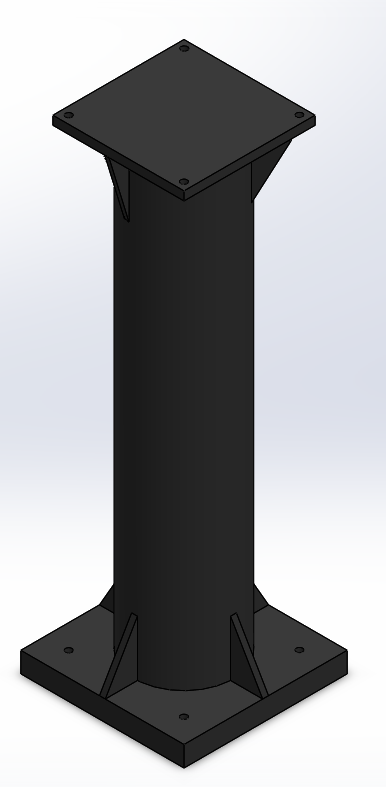
\includegraphics[scale=0.4]{BaseStructure}
	\caption{Base Structure}
\end{figure}

\vspace{0.6 cm}

\subsection {Design of Base Based On Strength}
\paragraph{Base Calculations}
This section discusses the process of calculating the following:
\begin{enumerate}
	\item Cylinder
	\begin{itemize}
		\item[--] Inner and outer diameters of the hollow cylinder.
		\item[--] The height of the cylinder.
	\end{itemize}

    \item Flanges
    \begin{itemize}
    	\item[--] Dimensions (length x width) of the 3 flanges
    	\item[--] The exact locations of the holes through which the bolts will be screwed
    	\item[--] Thickness of the flanges
    \end{itemize}

    \item Bolts
    \begin{itemize}
    	\item[--] Diameters of all bolts used in the installation and mounting of the base.
    \end{itemize}

    \item Ribs
    \begin{itemize}
    \item[--] Dimensions of the triangular ribs (height x width x thickness)
    \end{itemize}
\end{enumerate}

\vspace{0.5 cm}

\subsubsection{The inner and outer diameters of the cylinder}


Since the cylindrical body of the base undergoes different axial and torsional loads, it can be considered as a shaft.

\paragraph{Determining the cylinder diameters}
First attempt was to design the cylinder using the predefined mechanical properties of the commercial materials available in the market, to get the inner and outer diameters. After several weeks of research and calculation, the results were within the range of $10^{-2}$ to $10^{-3}$ mm, which is very small compared to the expected geometry of the cylinder, leaving us to pursue another manner of designing, based on the strength of material.

\paragraph {Design based on strength}
Second design attempt aimed to use the inner and outer diameters of the cylinders available in the market, to check whether the resulting shear stress would exceed the maximum allowable shear the material can withstand or not. The ASME code for this method is:

\begin{equation}
\tau_{allowable} = \frac{16}{\pi d^{3}_{o} (1-k^{4})} \sqrt{(k_{b} M_{b} + \frac{F_{a} d_{o} (1+k^{2})}{8})^{2} + (k_{t} M_{t})^{2}}
\end{equation}
where:
\begin{itemize}
	\item [--] Maximum shear stress the material undergoes upon action of axial and torsional loads: $\tau_{all}$
	\item [--] Combined shock and fatigue factors: $k_{b} = k_{t} = 1 : 2 $
	\textit{For safety purposes, the value of $k_{b}$ and $k_{t}$ constants is considered 2 in the calculations performed.}
    \item [--] Bending Moment: $M_{b} = F_{h} H$
	\item [--] Cylinder height: $H$
	\item [--] Horizontal shear force acting on the base: $F_{h}$
	\item [--] Torsional Moment: $M_{t}$
	\item [--] Axial force (tension/compression) acting on the base: $F_{a}$
	\item [--] Ratio of the inner to outer diameter: $k = \frac{d_{i}}{d_{o}}$
	\item [--] Maximum Allowable shear stress of a predefined specifications of a material, without keyways:
	$$ \tau_{all} = 0.3 \sigma_{y} $$
	$$ \tau_{all} = 0.18 \sigma_{u} $$
	\textit{These values shall be reduced by 25\% in the presence of keyways}
	\item [--] Maximum allowable shear stress of commercial steel, without keyways:
	$$ \tau_{all} = 55 MPa $$
\end{itemize}

\textit{The key is a machine element, that connects a rotating machine element to the shaft. It’s mainly used to prevent relative rotation between the two parts. A keyway is a slot in the shaft and the machine’s rotating element, in which the key is seated. In our case, there are no keyways used, because the base is built to be held stationary.}
\vspace{0.3 cm}
\newline Using the following values of loads acting on the foundation mentioned in the KR AGILUS specification manual:
\begin{figure}[H]
\begin{center}
	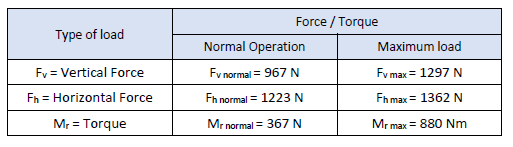
\includegraphics[scale = 0.95]{Loads}
\end{center}	
\end{figure}

Using steel A37 with the following specifications:
\begin{itemize}
	\item[--] Yield Strength: $\sigma_{y} = 235 MPa$
	\item[--] Ultimate Tensile Strength: $\sigma_{u} = 360 MPa$
\end{itemize}

The max allowable shear stress is:
$$ \tau_{all} = 0.3 (235) = 70.5 MPa $$
$$ \tau_{all} = 0.18 (360) = 64.8 MPa $$
\vspace{0.3 cm}
\newline The following table shows the different values of diameters available in market, along with the corresponding resulting shear stress:
\begin{figure}[H]
	\begin{center}
		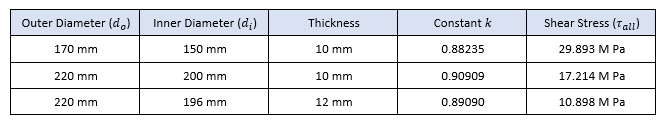
\includegraphics[scale = 0.95]{CalculationsResults}
	\end{center}	
\end{figure}

Thus, by comparing the previous values of resulting shear stress to the minimum value of the maximum allowable shear stress the material can withstand, 64.8 MPa, we find that any of the alternatives would be suitable for manufacturing the cylinder.

\bigskip

\subsubsection{Bolts’ diameters}
\begin{itemize}
	\item Lower flange
\end{itemize}

To get the diameters of the used bolts, we need to calculate the tension forces acting on them first. 
\begin{equation}
M_{b} = 2 F_{1} r_{1} + 2 F_{2} r_{2} = H F_{h}
\end{equation}
$$\frac{F_{1}}{r_{1}} = \frac{F_{2}}{r_{2}}$$
$$ F_{1} = F_{2} \frac{r_{1}}{r_{2}}$$
Substituting $F_{1}$ in equation (1.2), we get:
\begin{equation}
H F_{h} = 2 F_{2} (\frac{r_{1}^{2}}{r_{2}} + r_{2})
\end{equation}

Where $r_{1}$ and $r_{2}$ are the distances from one edge of the flange to the first pair of bolts, and the second pair respectively, as shown in figure below.
\begin{figure}[H]
\begin{center}
	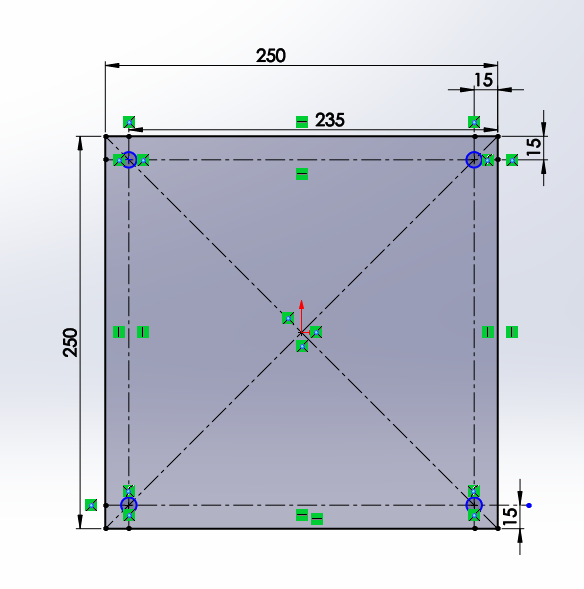
\includegraphics[scale=0.5]{R1R2}
	\caption{values of $r_{1}$ and $r_{2}$}
\end{center}	
\end{figure}

\textit{Notes:} 
\begin{itemize}	
\item[--]  The values of dimensions of the flanges and distances $r_{1}$ and $r_{2}$ are defined based on the assumption that the bolts used in the lower flange is 10 mm, until reasonable results are obtained using try and error.
\item[--] All dimensions mentioned in this chapter are measured in mm.
\end{itemize}



If the diameter of bolts holding the lower flange is 10 mm, and the area of the flanges is (250x250) $mm^{2}$, then the values of $r_{1}$, $r_{2}$ are 15 mm and 235 mm respectively, as shown in the figure below.
\newline Substituting the values of $M_{b}$, $r_{1}$, and $r_{2}$, we get:
$$ F_{2} = 2308.89 N $$
Repeating the previous steps by substituting $F_{2}$ with $F_{2}$, we get:
$$ F_{1} = 147.376 N $$

For safety purposes, the design of the bolts will be based on the larger tension force, $F_{2}$.
After obtaining the tensile forces on the bolts, the tensile strength ($\sigma_{t}$) should be calculated to check for safety:

\begin{equation}
\sigma_{t} = \frac{F_{t}}{\frac{\pi}{4} d^{2}}
\end{equation}

For 10 mm bolts diameter, and the previously calculated tensile force, we get:
$$ \sigma_{t} = \frac{2308.89}{\frac{\pi}{4} (0.01)^{2}} = 29.398 MPa $$ 

Taking in consideration a factor of safety, and checking for the maximum tensile strength the material can undergo before failing:
$$\sigma_{t} = \frac{\sigma_{y}}{F.S.} = \frac{235}{3} = 78.33  MPa$$
The resulting tensile stress is less than the maximum allowable tensile stress, hence, the previous design is safe.
\newline It was previously mentioned that we used commercial materials available in the market. The manufactured steel sheets are of thickness 15 mm, calculations need to be made to check for safety according the maximum shear and bearing stresses.
\newline The horizontal shear force exerted on the base will be acting on the bolts as well, however, it is negligibly small because it’s mostly eliminated by the existence of friction between the two steel flanges it holds. Moreover, the moment resulting from tightening the bolts produces an axial force eliminating the axial load acting on the base.

\begin{figure}[H]
	\begin{minipage}{0.5\textwidth}	
		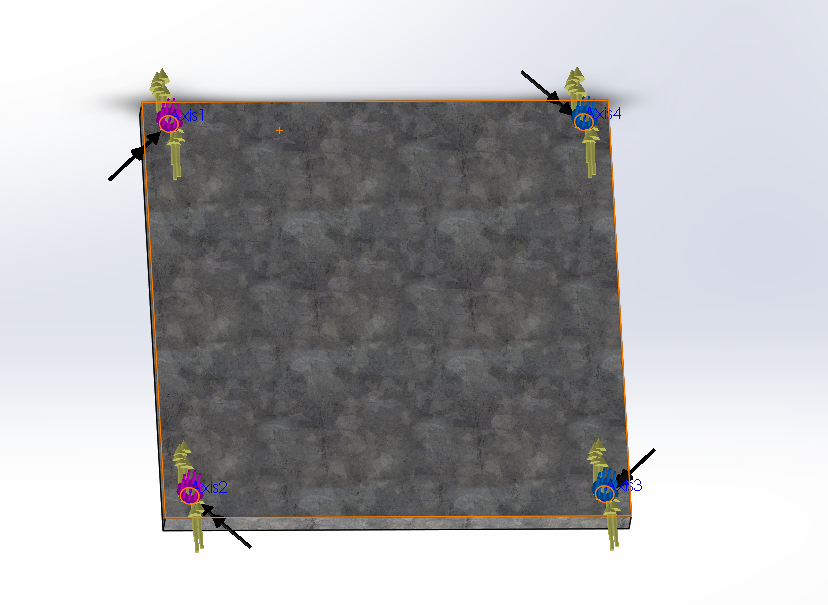
\includegraphics[scale=0.35]{CombinedForces1}
	\end{minipage} \hfill
	\begin{minipage}{0.6\textwidth}
		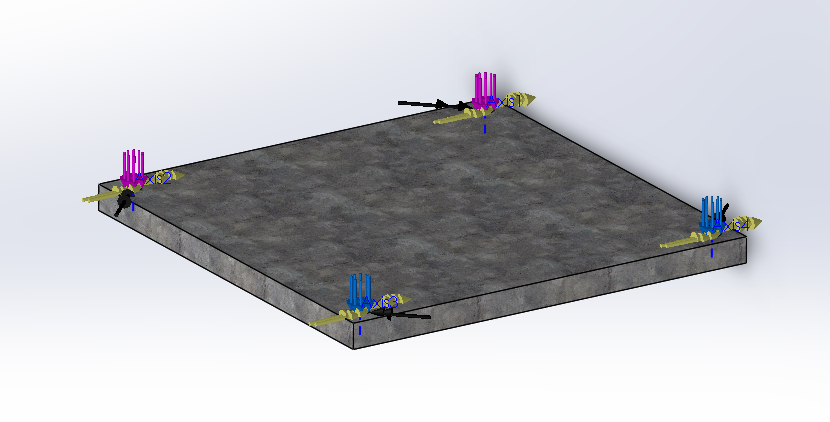
\includegraphics[scale=0.5]{CombinedForces2}
	\end{minipage}
	\begin{center}
		\caption{Forces acting on bolts. Black arrows: $F_{tr}$ , purple: $F_{a}$, green: $F_{h}$ }
	\end{center}
\end{figure}

\begin{equation}
F_{total} = \sqrt{(\frac{F_{h}}{4})^{2} + (F_{tr})^{2} + 2 F_{tr} F_{h} cos \theta}
\end{equation}

\begin{equation}
F_{tr} = \frac{M_{t}}{4 R}
\end{equation}

Where R,which  is the radius of perimeter, has a value of 176.78 mm  as shown in figure below.

\begin{figure}[H]
	\begin{center}
		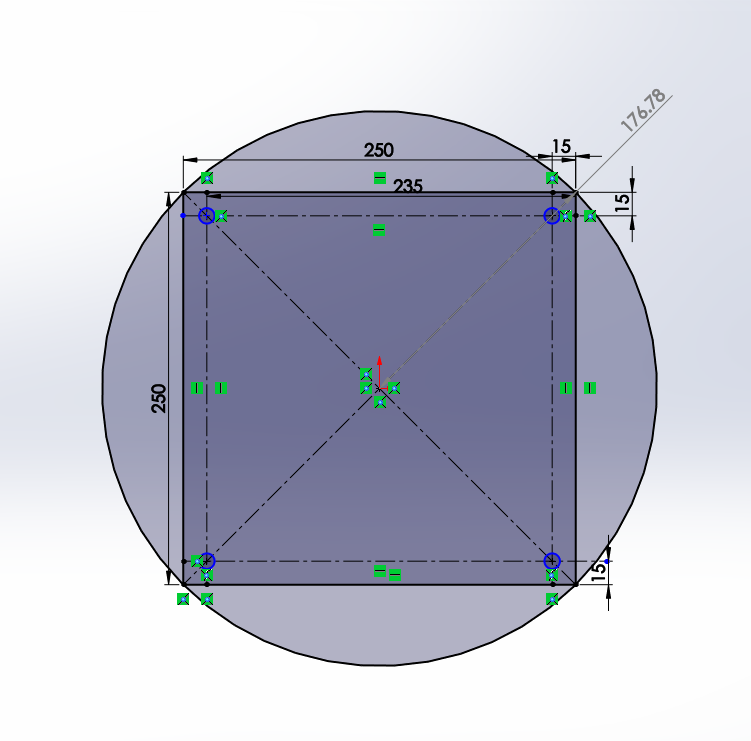
\includegraphics[scale = 0.3]{R}
		\caption{value of R}
	\end{center}
\end{figure}

$$ F_{tr} = \frac{880}{4 (0.1768)} $$
$$ F_{total} = \sqrt{(\frac{1362}{4})^{2} + (\frac{880}{4 (0.1768)})^{2} + (2\frac{1362(880)}{4(4)0.1768} cos 45)} = 1504.5 N $$

Checking for safety in terms of the bearing stress:
\begin{equation}
\sigma_{br} = \frac{F_{total}}{d_{b} t} = \frac{1504.5}{0.01(0.015)} = 10.03MPa
\end{equation}

By comparison to the maximum allowable bearing stress, we find that both of the predetermined bolt diameter (10 mm), and the flanges thickness are verified to be safe and suitable, as following:

\begin{equation}
\sigma_{br} = 1.2 \frac{\sigma_{y}}{F.S.} = \frac{1.2(235)}{3} = 94 MPa
\end{equation}

Checking on the maximum shear stress exerted on the bolts by the combined forces, we get:

\begin{equation}
\tau = \frac{F_{total}}{\frac{\pi}{4} (d_{b})^{2}} = \frac{1504.5}{\frac{\pi}{4} (0.01)^{2}} = 19.156 MPa
\end{equation}
Comparing it to the maximum shear stress the bolts can stand which is 64.8 MPa since it's made of the steel-37 as well, we can conclude that this is a safe design in terms of the bolts diameters, flanges dimensions, and cylinder diameters.

\bigskip

\subsubsection{Upper Flange}
The upper flange holds the robot base motor, using the bolts provided with the robot. The flange was designed to have an area of (230x230) $mm^{2}$, with the locations of 4 bolts holding the robot taken from its base.

\bigskip

\subsubsection{Ribs}
The ribs are made of the same sheet of which the flanges are made of, with a thickness of the ribs is 10 mm. 
\newline There isn’t an exact way of calculating the height and width of the triangular ribs. After discussing the matter with several machine design doctors, we concluded that the ribs’ width should cover the length from the cylinder surface to the edge of flange, resulting in a width of 55 mm, while the height is 100 mm.


\newpage

\subsection{Base Manufacturing \& Installation }

\subsubsection{Manufacturing}

Several materials can be used to manufacture the body of the base, such as AISI 1010 \& AISI 1010 carbon steel, SAE 304 stainless steel, etc., all of which the mechanical properties are predefined. However, the available material in the market was steel 37, which has the following mechanical specifications:

\begin{itemize}
	\item[--] Yield Strength: $\sigma_{y} = 235 MPa$
	\item[--] Ultimate Tensile Strength: $\sigma_{u} = 360 MPa$
\end{itemize}


The calculations performed on this material are proven to be safe and suitable to our designed base geometry. 
\vspace{0.2 cm}
\newline The squared, upper and lower flanges are made of a 15mm thick steel-37 sheet, and holes were drilled in the designated locations shown in the sketches below. The flanges are then welded to the cylindrical body of the base. It’s worth mentioning that the dimensions of the manufactured base are larger than those calculated, this is due to different manufacturing and safety purposes, the final dimensions manufactured are illustrated below.
\begin{figure}[H]
\begin{center}
	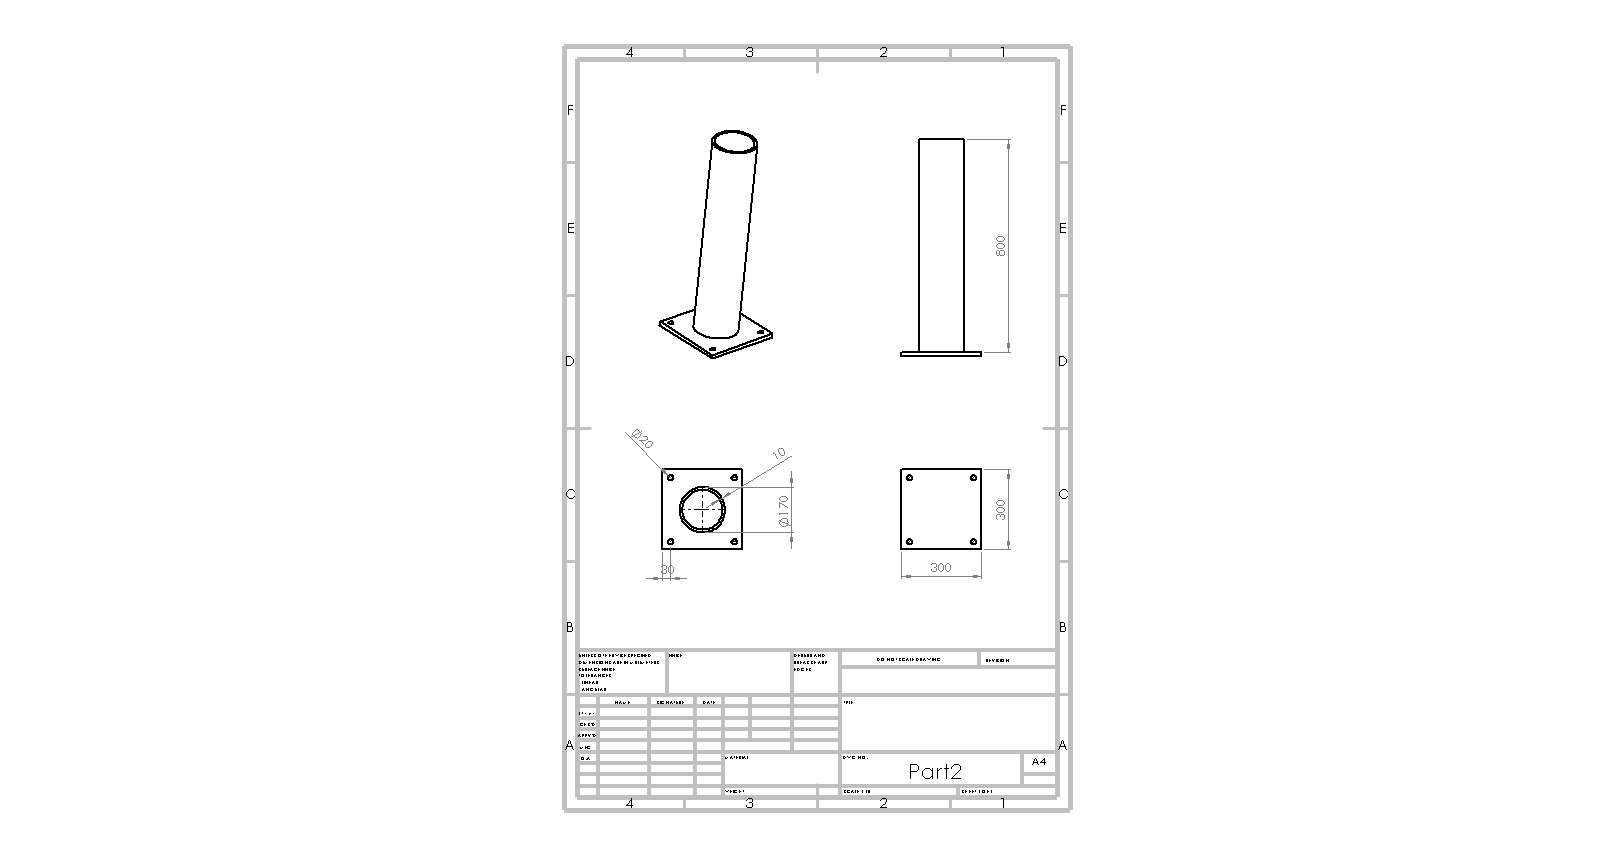
\includegraphics[scale=0.5]{BaseDim}
	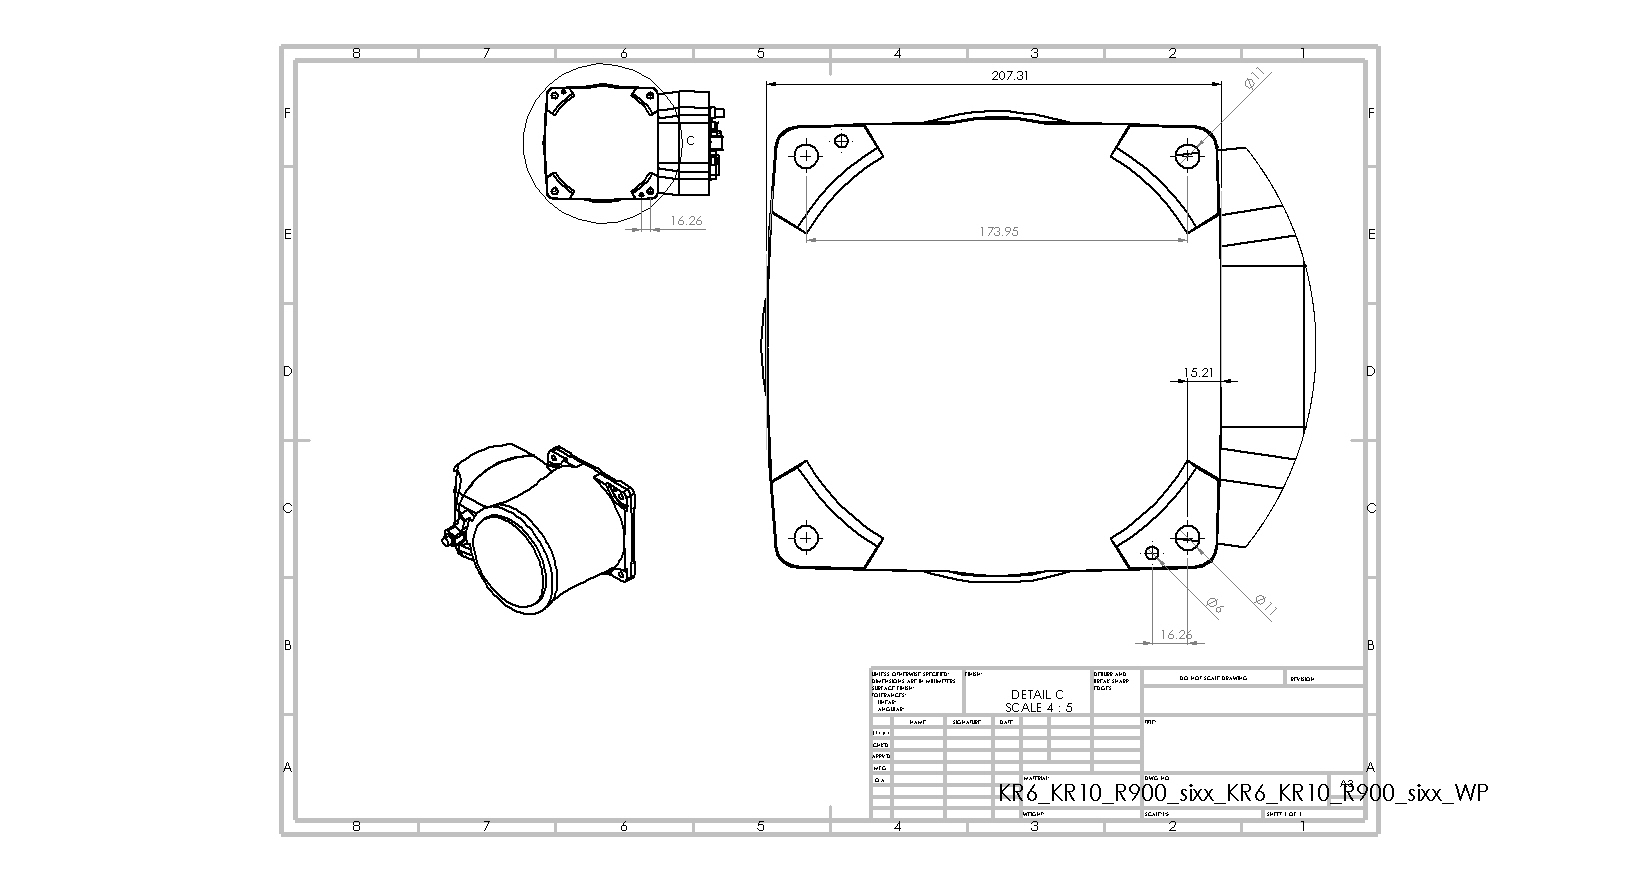
\includegraphics[scale=0.5]{BaseDim2}
	\caption{Final dimensions manufactured base}
\end{center}
\end{figure}


For the ribs to be welded, the base needs to be cleaned of any accumulated rust, it is then taken to undergo different machining steps, using a lathe machine. Next, it is painted in black to match the robot colors.
\newline \figurename{1.4} illustrates different stages of manufacturing.

\begin{figure}[H]
\begin{center}
	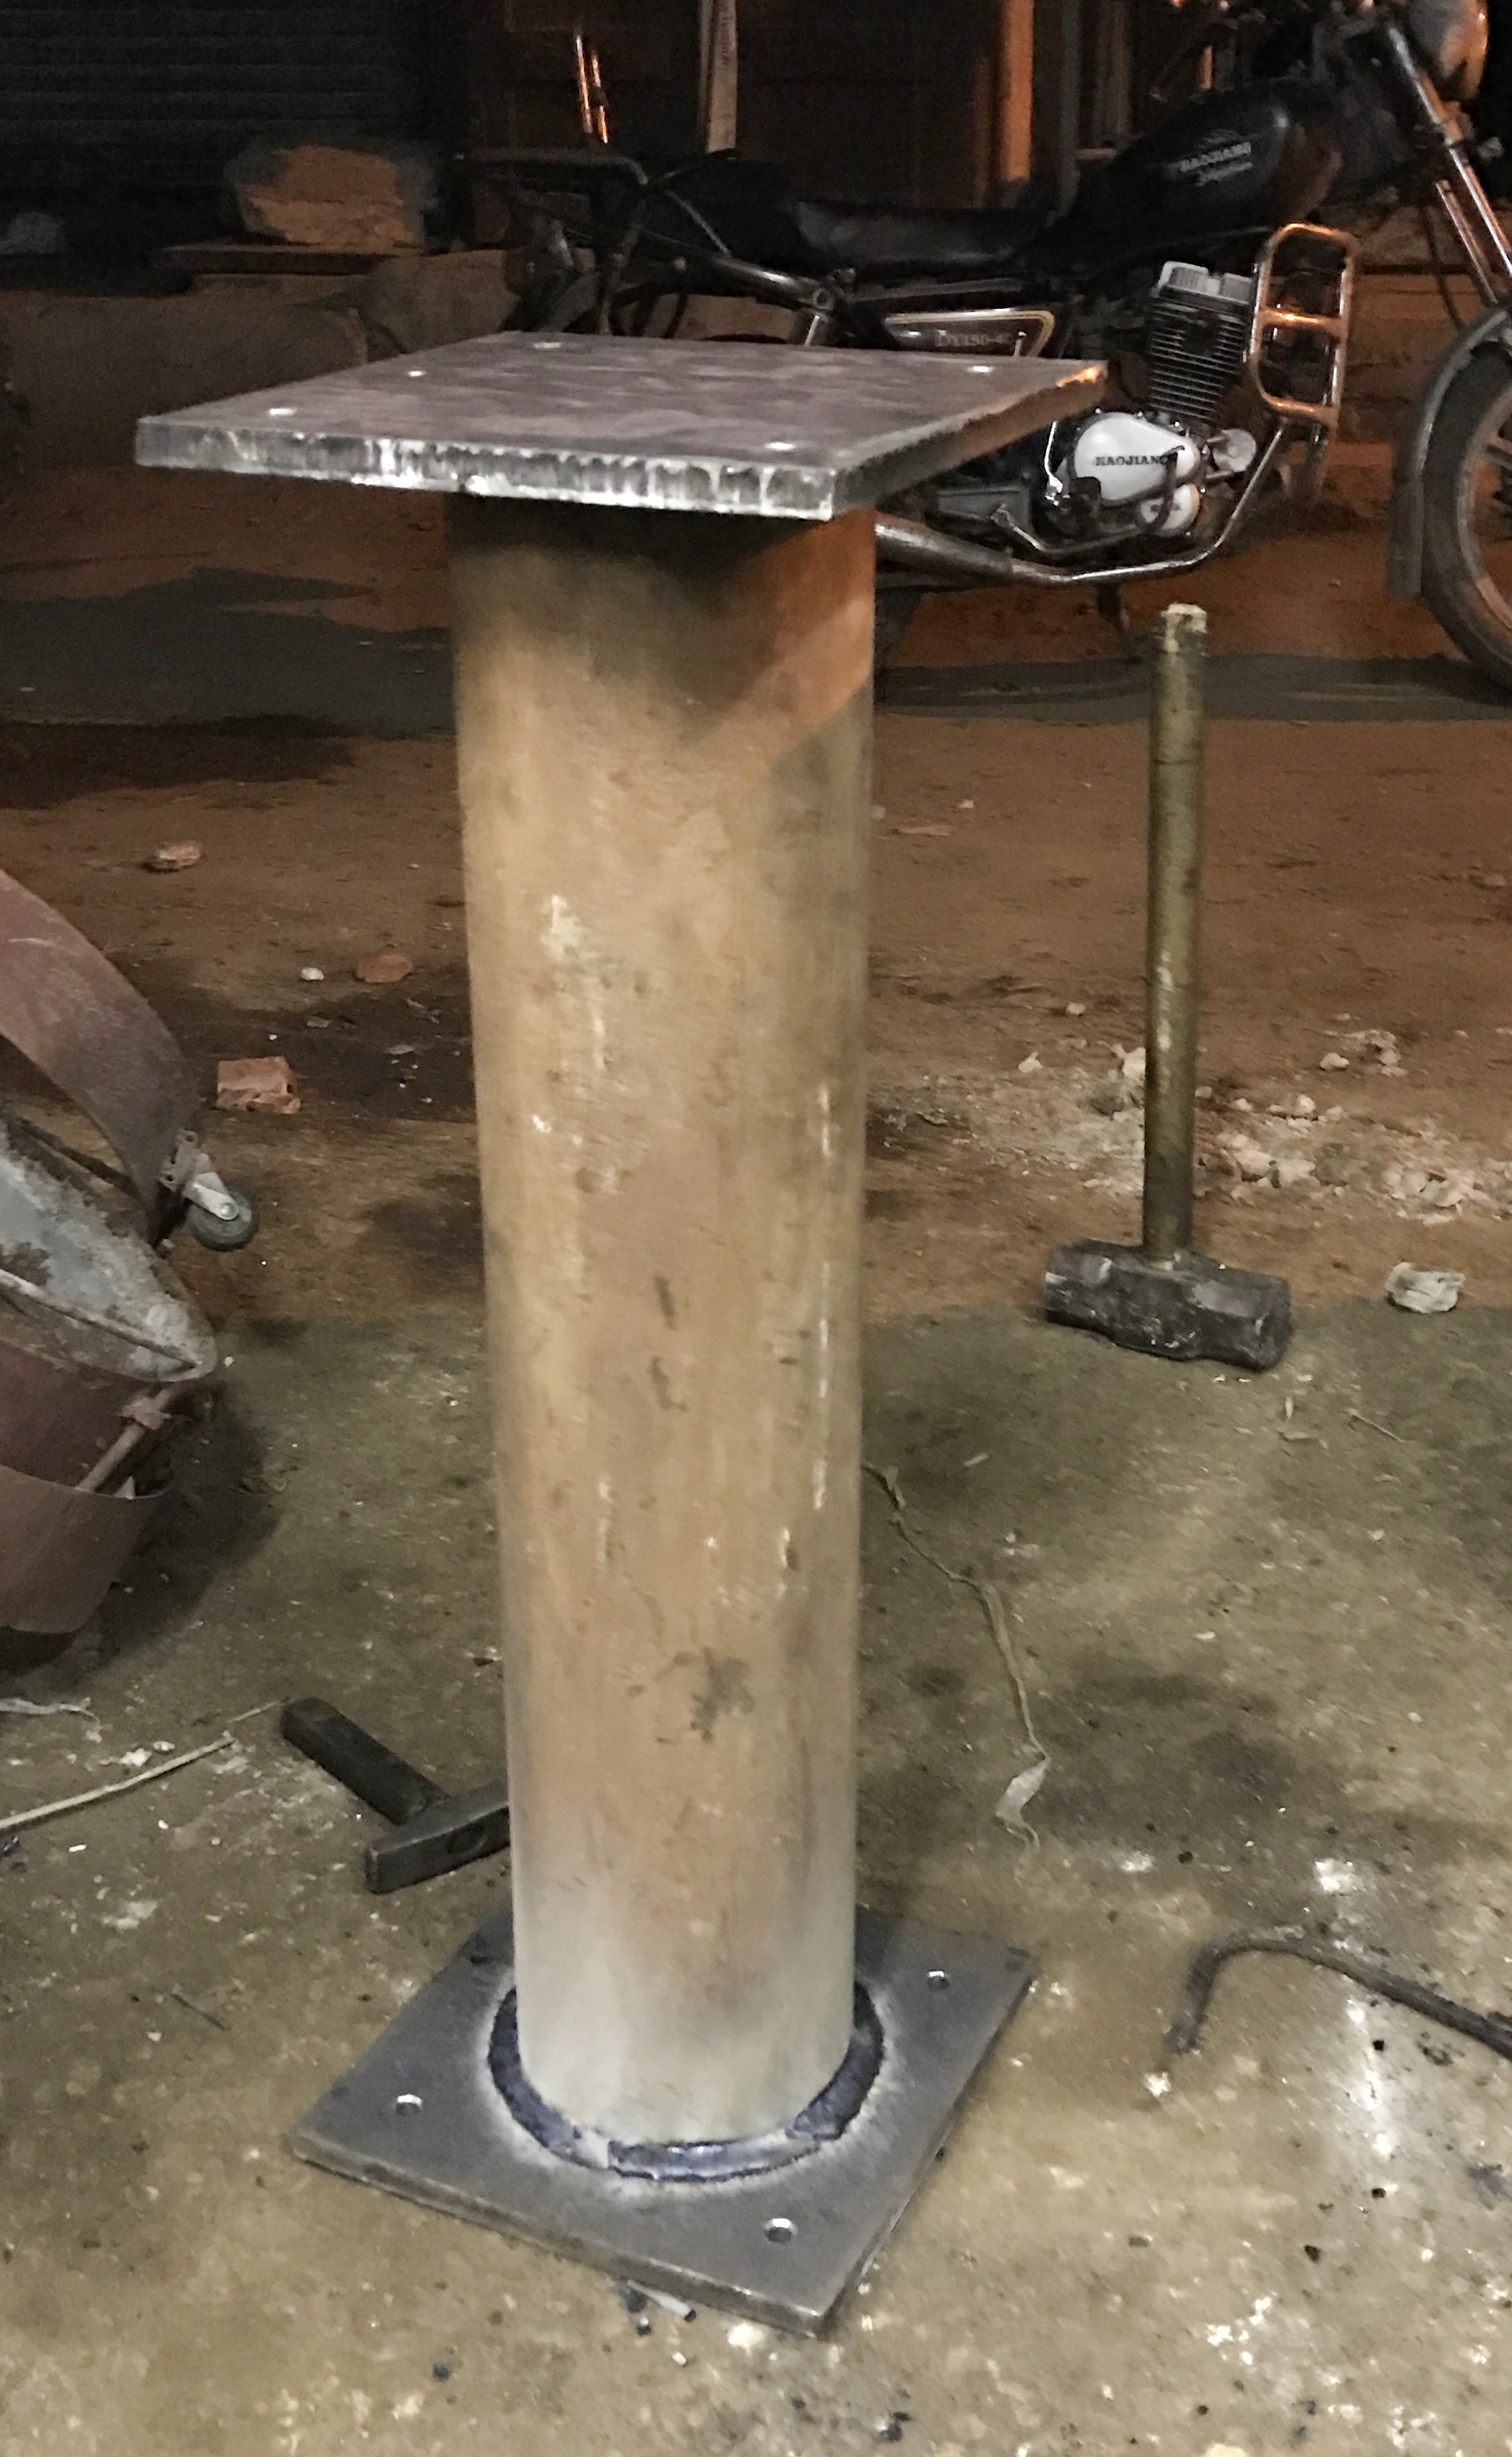
\includegraphics[scale=0.055]{WeldedFlanges}
	\includegraphics[scale=0.04]{Lathe}
	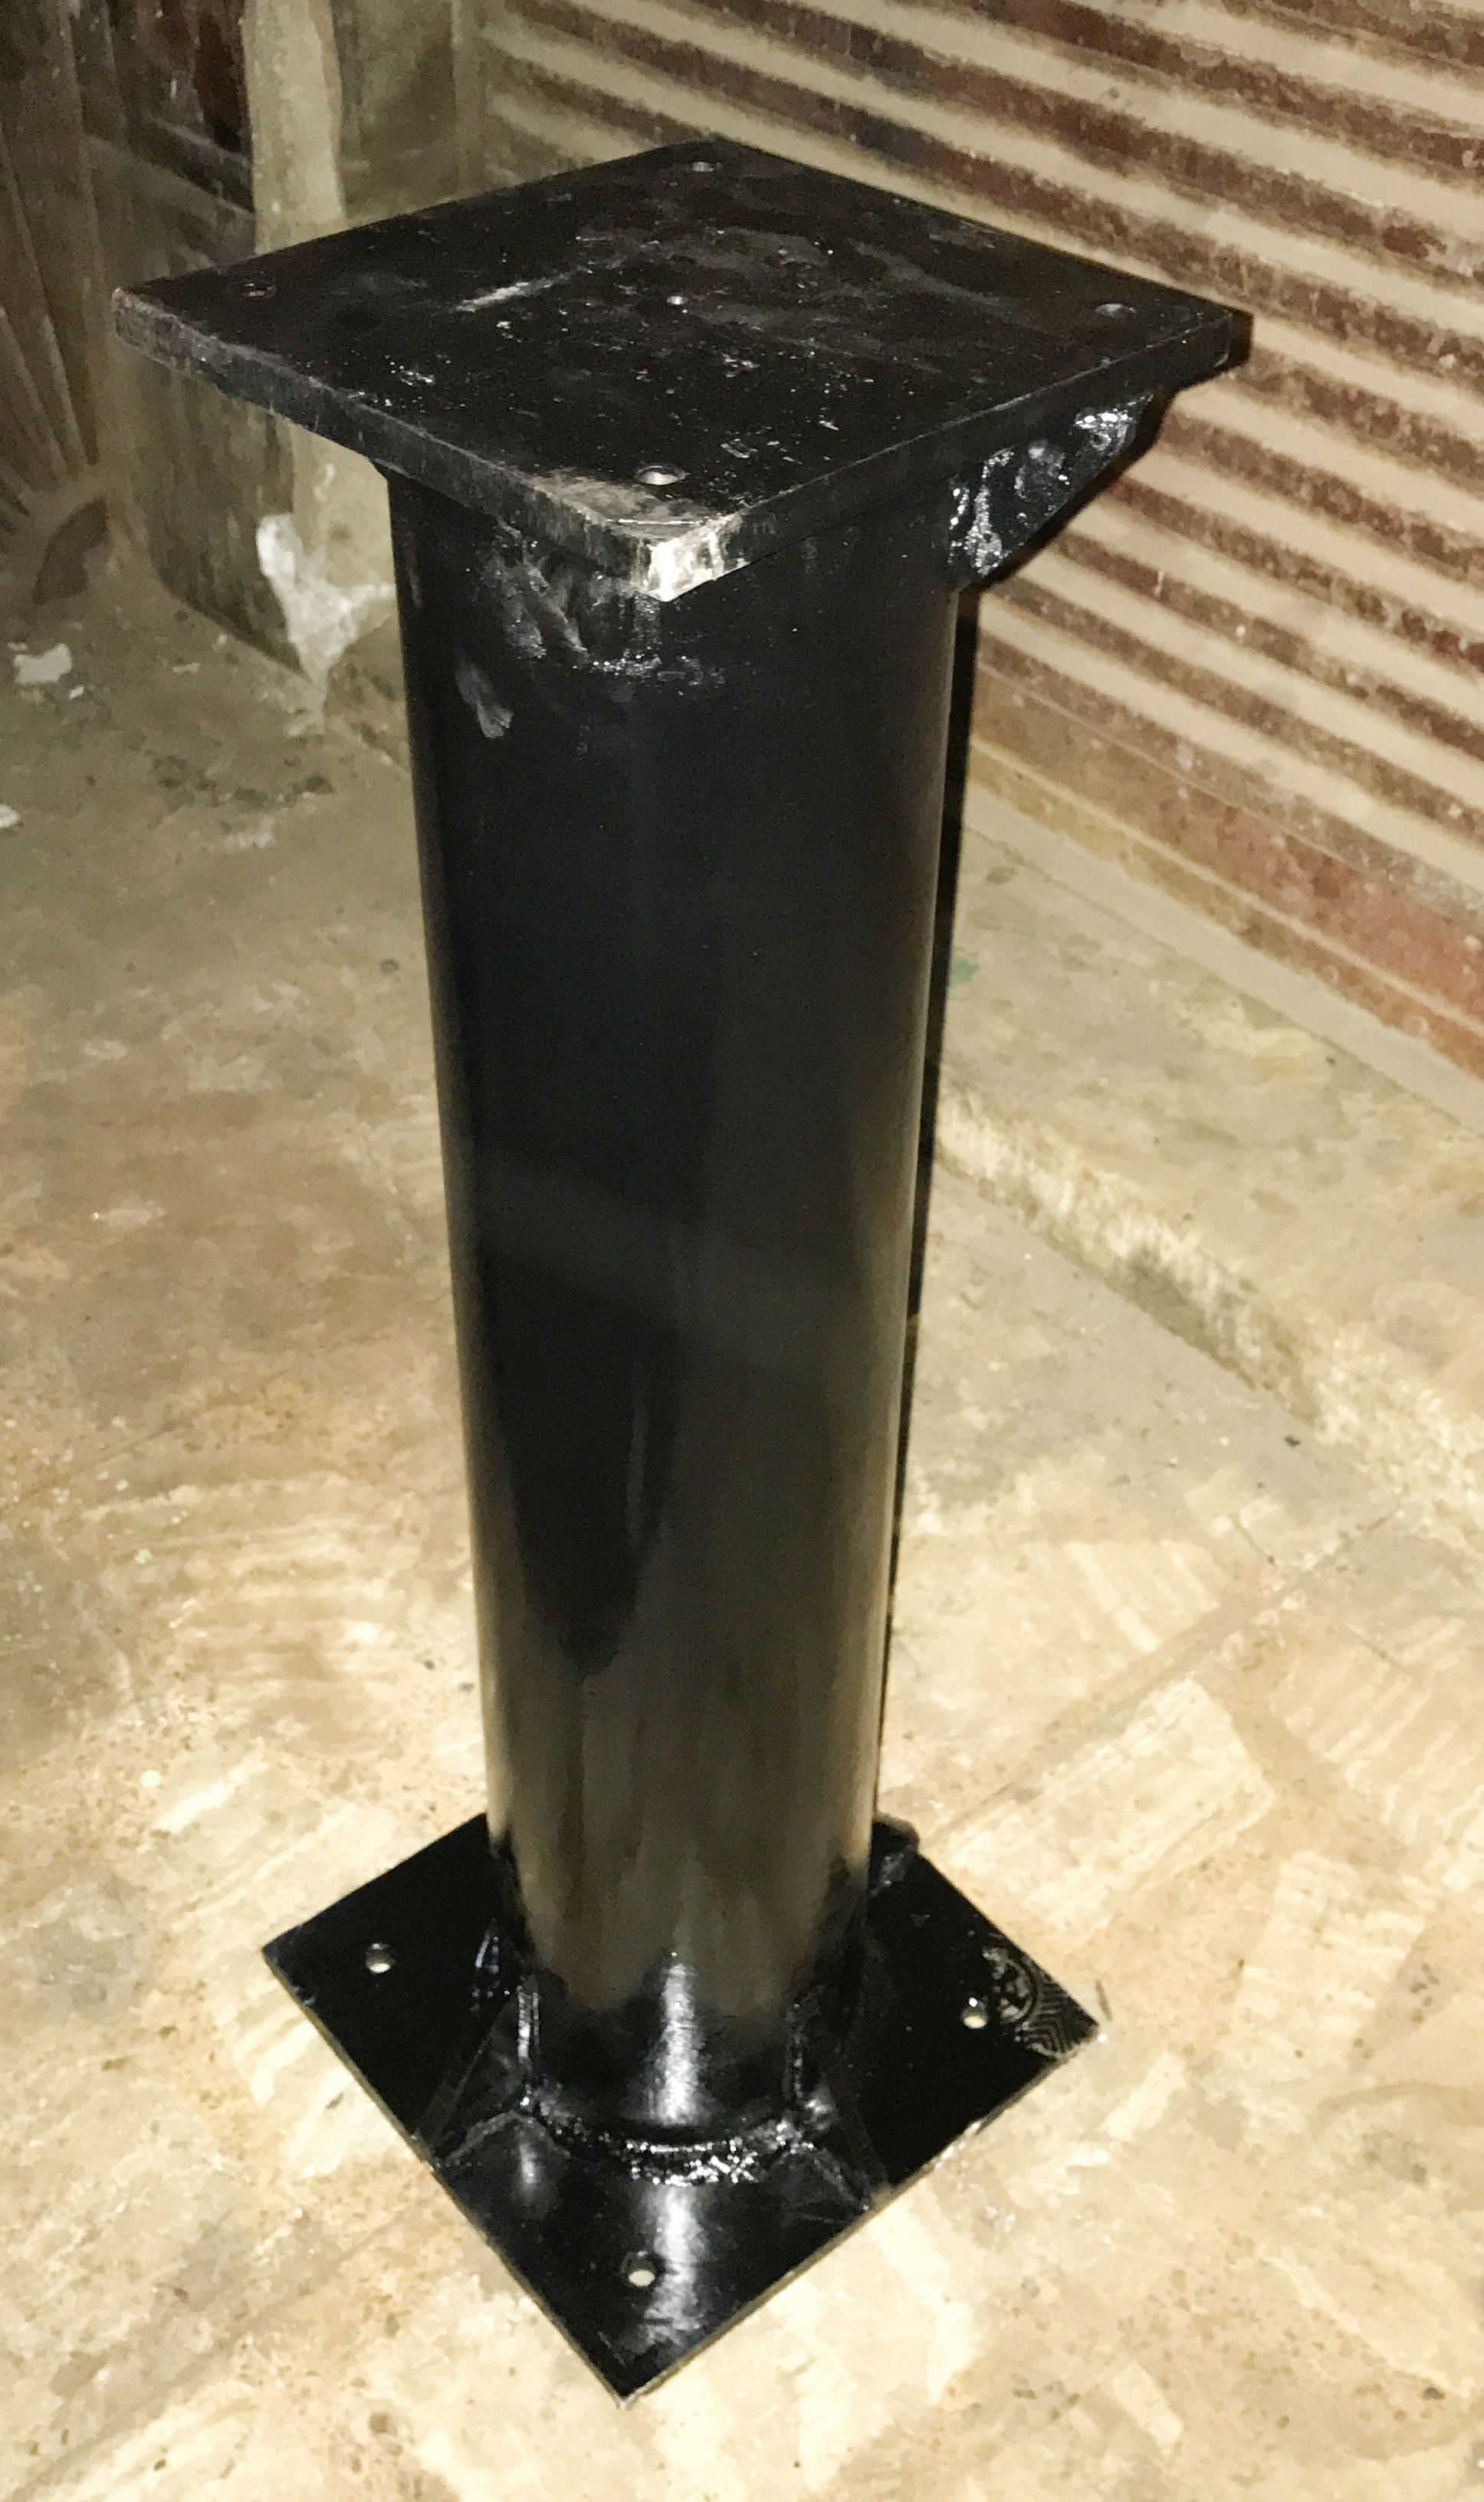
\includegraphics[scale=0.049]{PaintedBase}
	\caption{Manufacturing and Machining of the base}
\end{center}
\end{figure}

\subsubsection{Installation}

The following steps clarifies the process of installing the robot base:
\begin{enumerate}
	\item The exact location of the base is chosen according to the safe operating range of the robot, mentioned in the KR AGILUS sixx specification manual.
	\item Remove the ceramic plate. The number of plates removed depends on the area of the base and the ceramic plate itself, in our case, only one plate was removed.
	\item Scrape the sand and cement layers beneath the ceramic until you reach the concrete, it can be recognized when a layer of gravels appears.
	\item Drill the holes, in which the dowel rods will be placed, in the predesigned positions in the concrete. For this design, seven holes were drilled, however, the number of dowels depends on the design.
	\item Make a mixture of sand, gravels, cement and anabond adhesive agent to mold a new concrete layer, and keep mixing until it’s consistent.
	\item Pour in the concrete mixture on top of the pre-existent one, while the dowels are placed, and wait for 2 days to ensure that it’s completely solidified.
	\item Remove the dowels and start screwing the bolts.
    \item Start mounting the first flange. Use a bubble level to check if it lies in a perfectly horizontal position, if not, you must scrape the newly molded concrete layer until it’s even. 
	\textit{\newline Note: Even out the newly molded concrete once it dries, this would help you to avoid such issues in further steps.}
	\item Mount the base, then move the robot carefully until it’s placed on it in the right orientation.
\end{enumerate}

\figurename{1.5} illustrates different stages of the previously explained installation process.

\begin{figure}[H]
\begin{center}
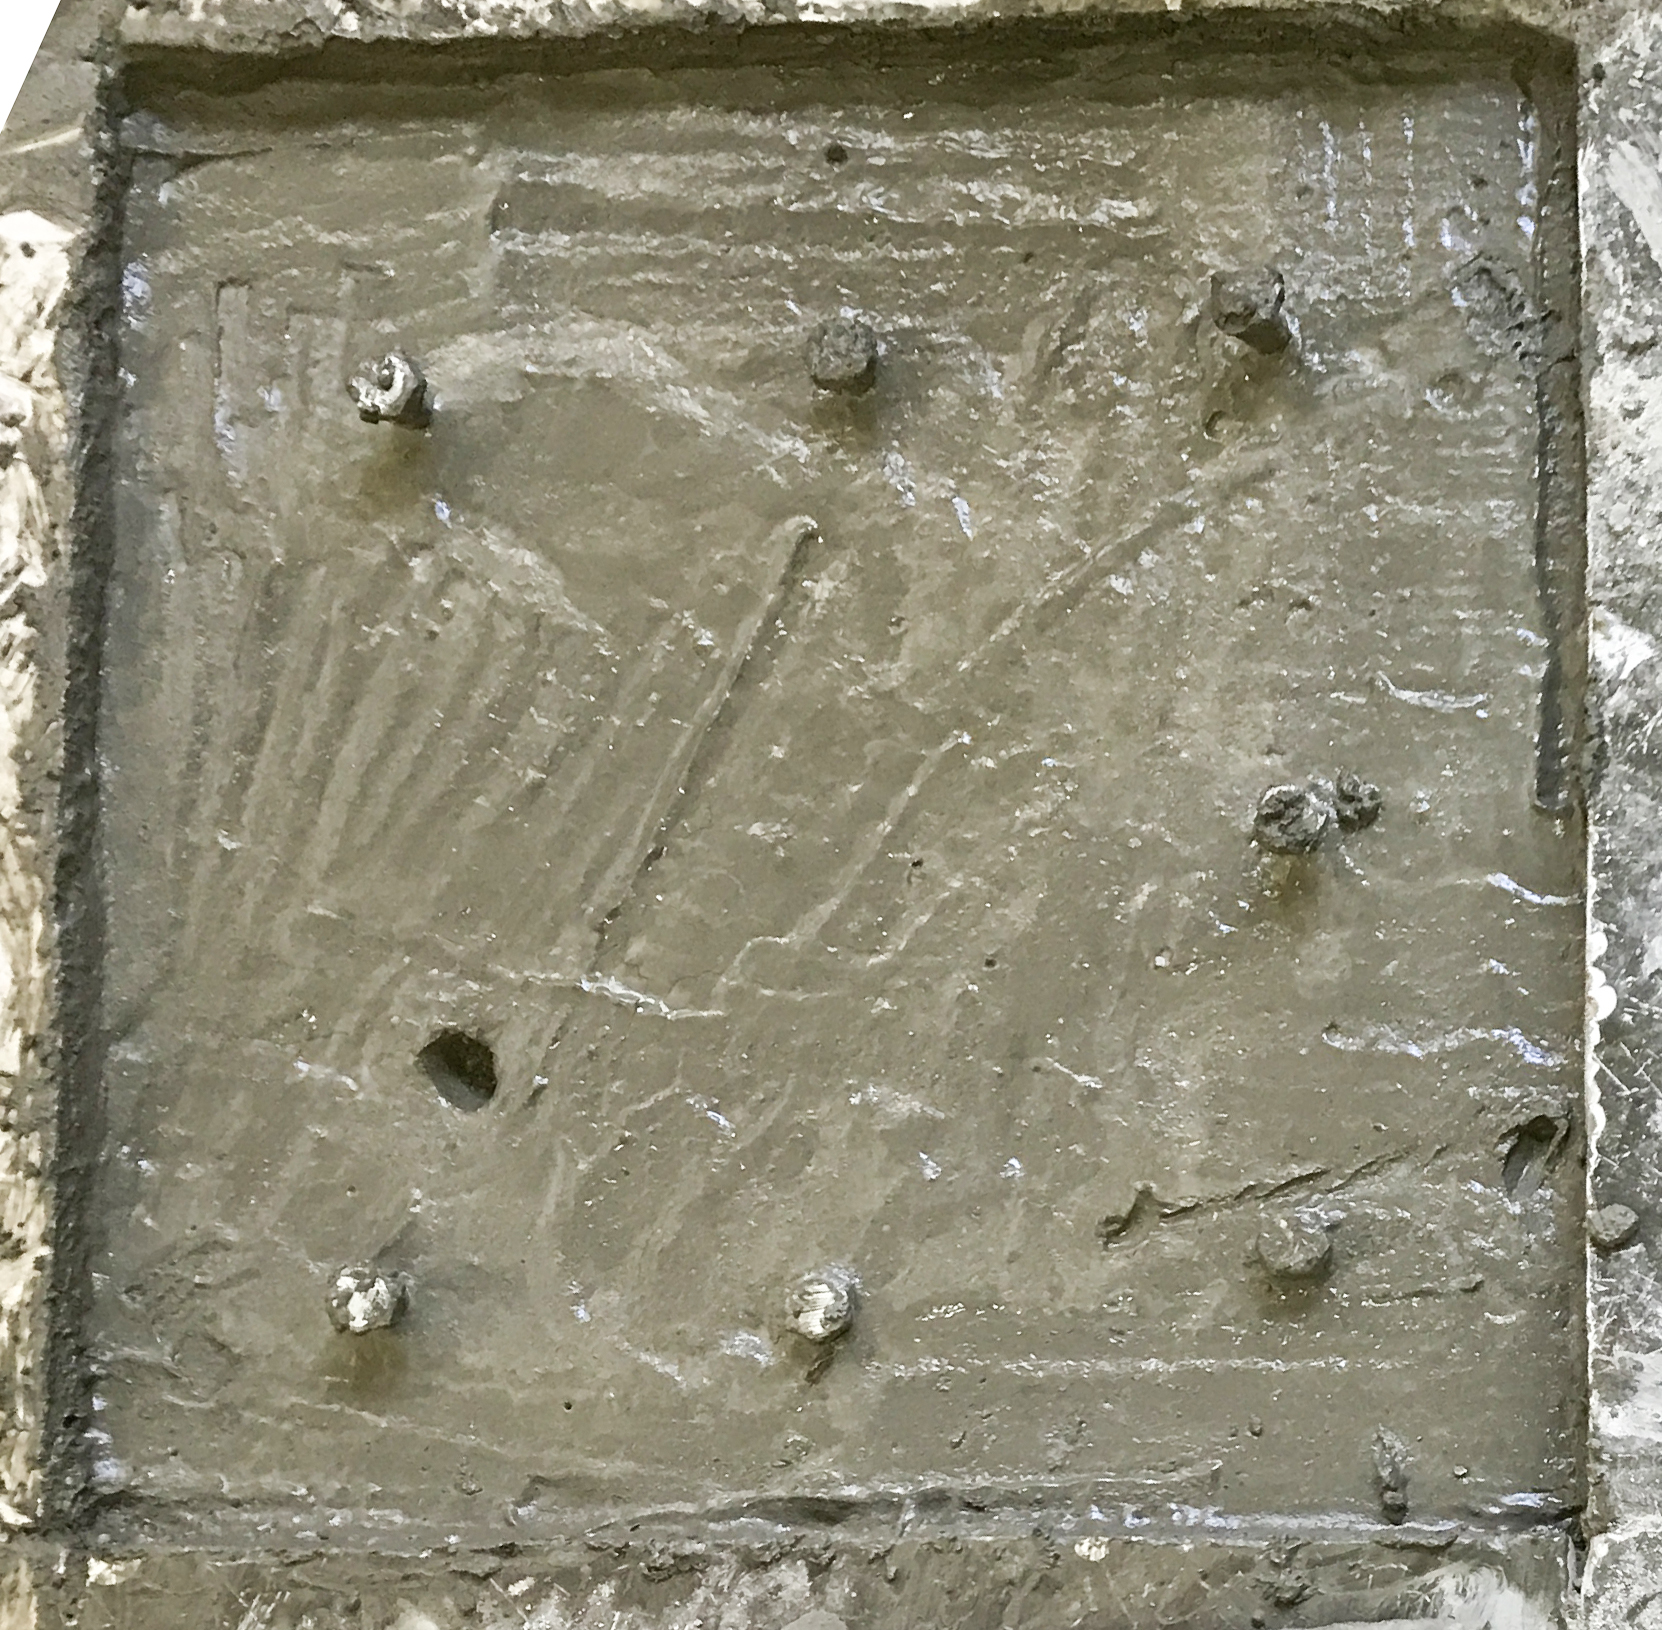
\includegraphics[scale=0.098]{MoldedConcrete}	
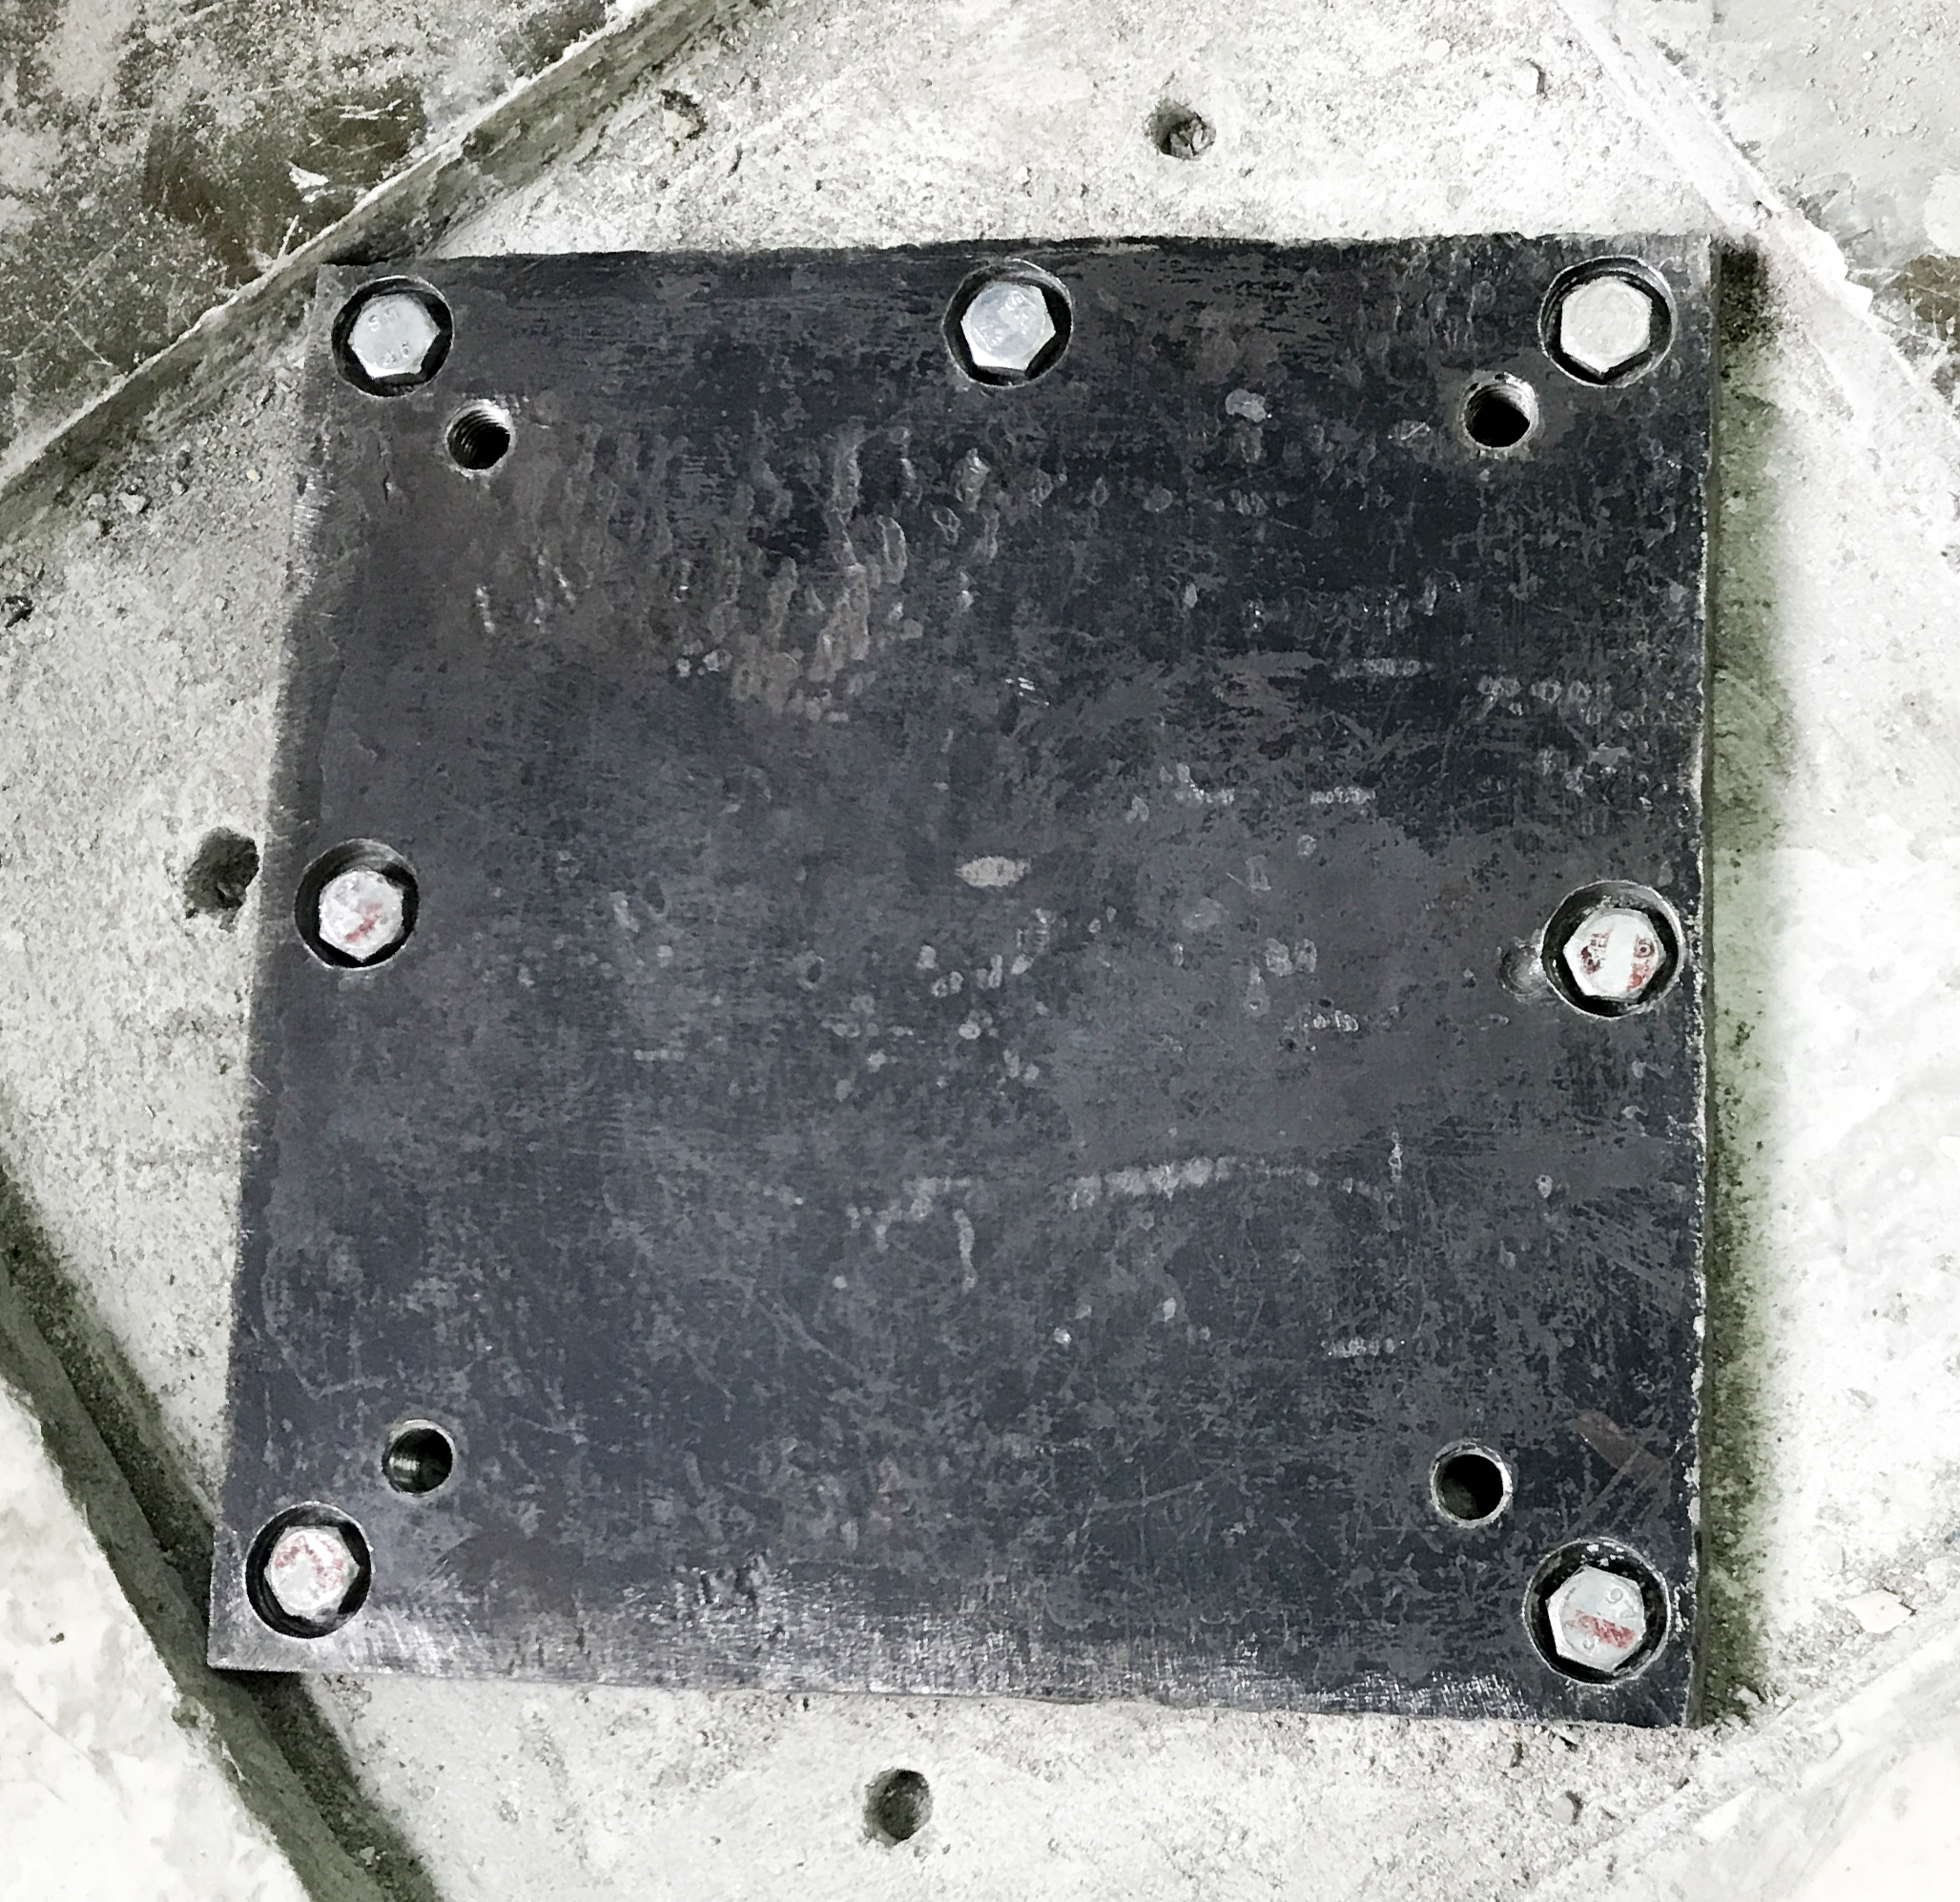
\includegraphics[scale=0.08]{FirstFlange}
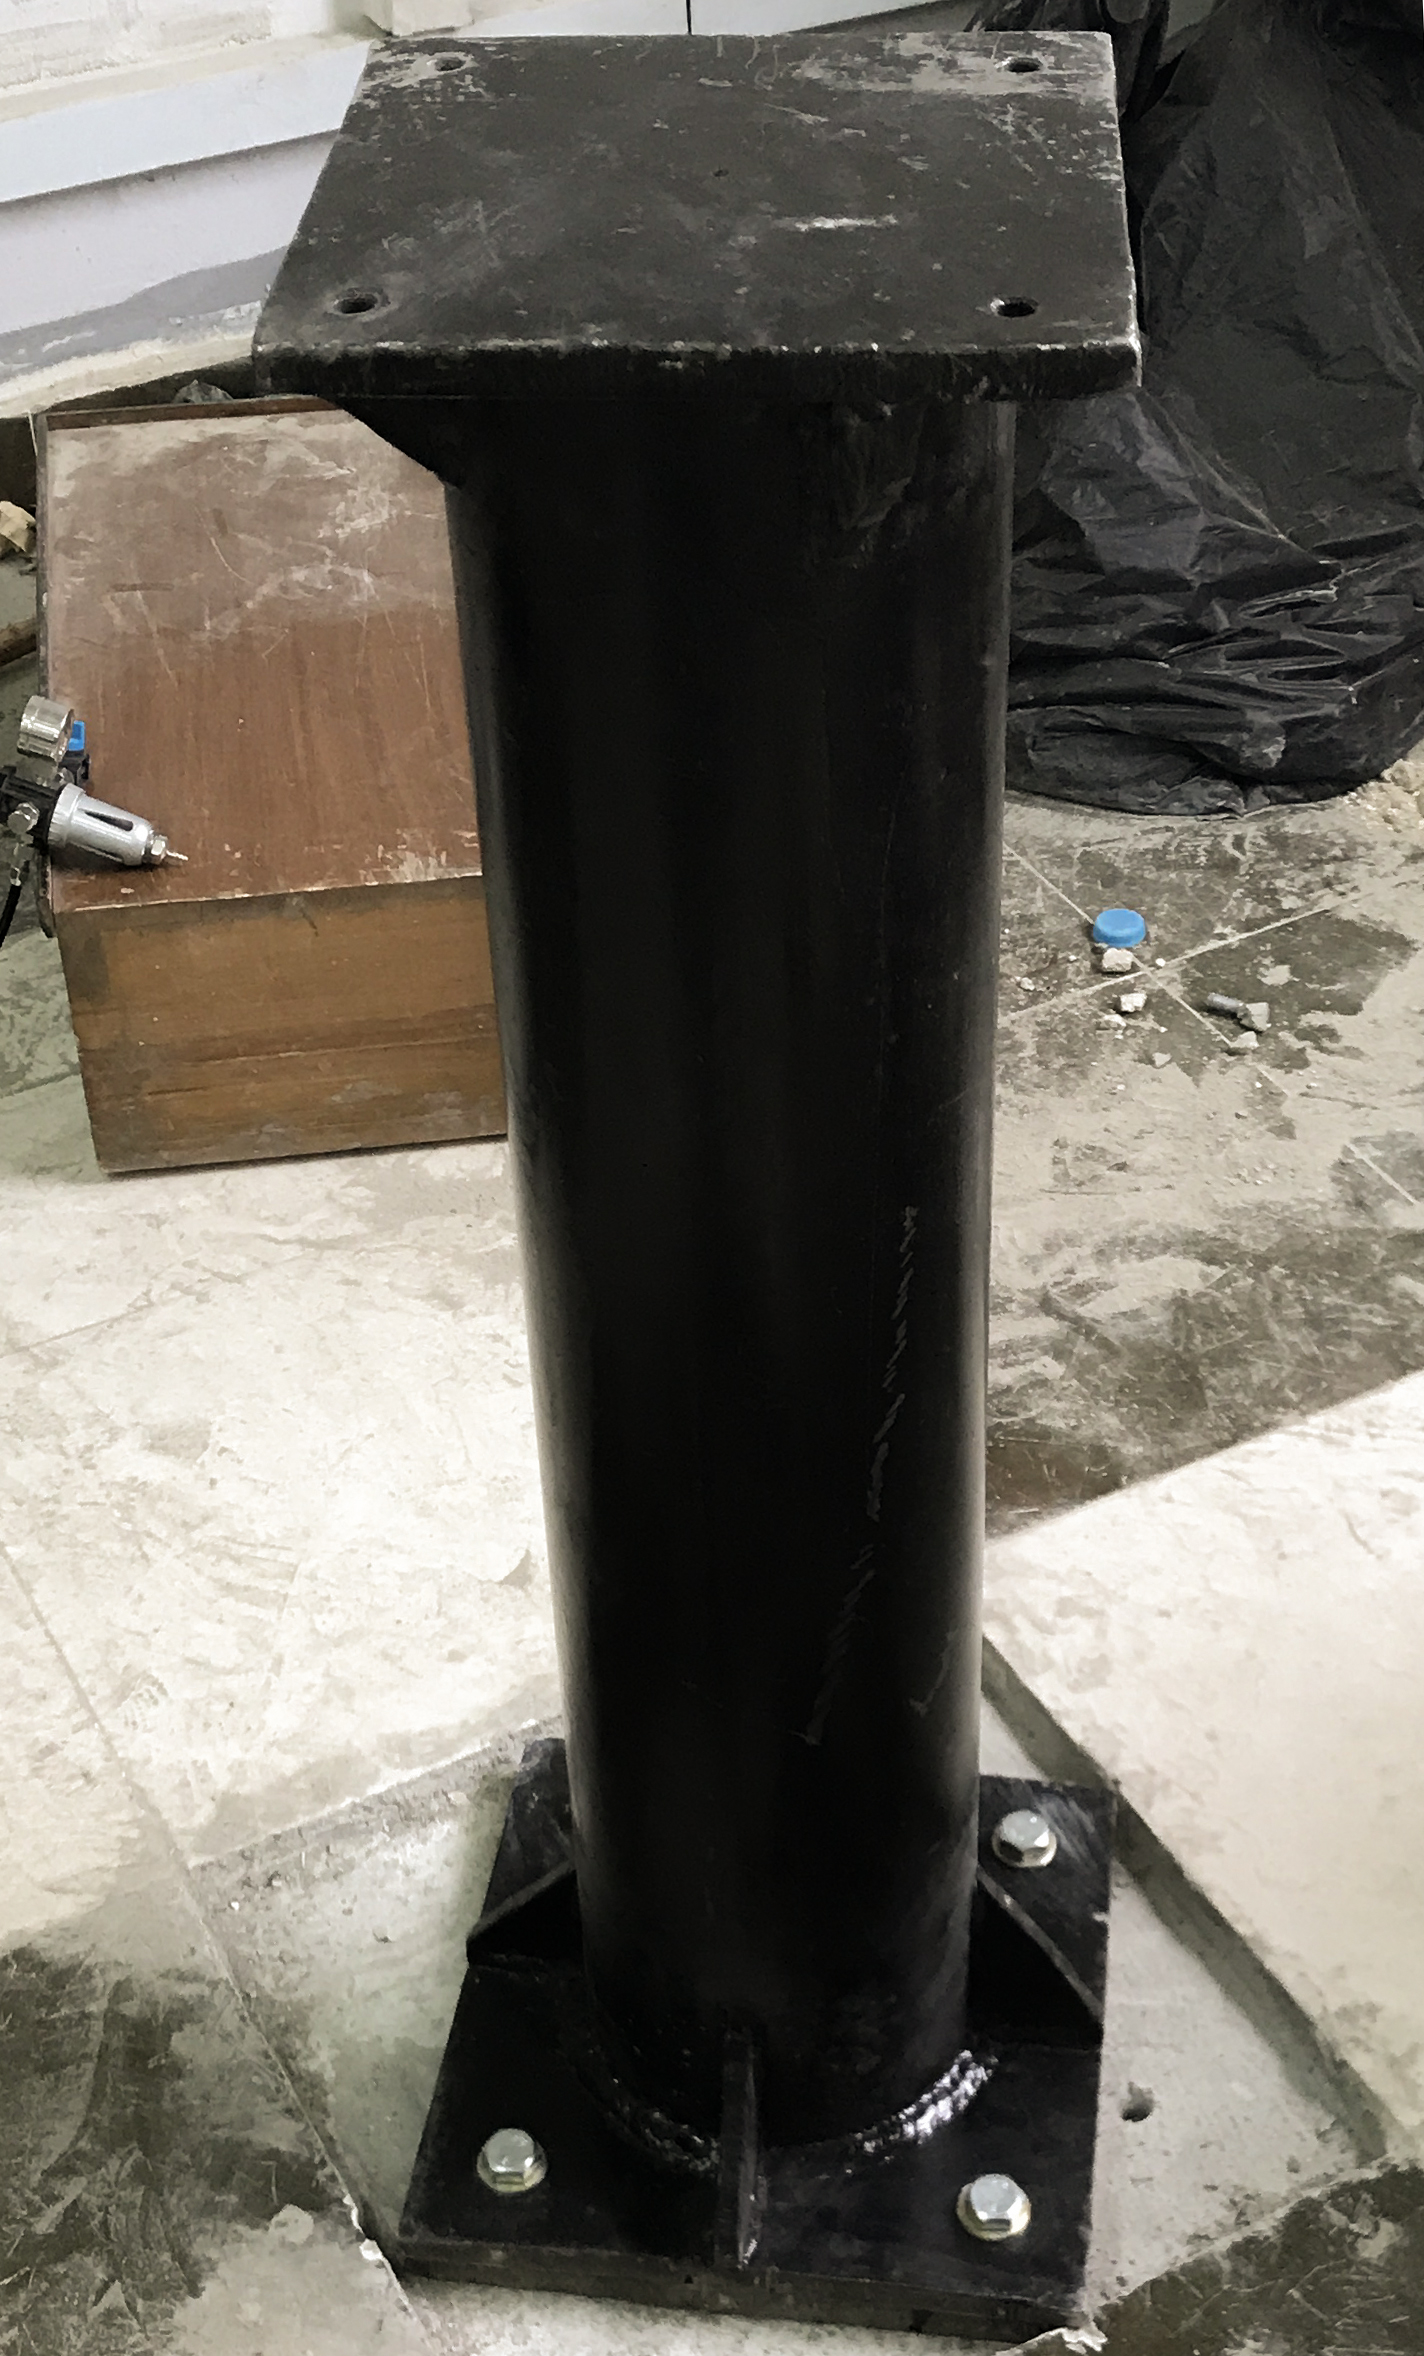
\includegraphics[scale=0.08]{MountedBase}
\caption{Base Installation}
\end{center}
\end{figure}



\newpage
\subsubsection{CAD Analysis Performed on Base}
For the purpose of our study, SolidWorks was used as a CAD software, as it contains solid modeling, motion studies, Simulation PhotoView 360, e-drawing and many other features that were used to obtain a complete CAD model for KR6 r900 sixx KUKA arm. 
\newline SolidWorks simulation is used to make a stress and strain analysis on designed base model to have a verification on the calculated dimensions of the base before starting fabricating it. Static study is used to perform this analysis as we use maximum loads acting on foundation base 


\begin{figure}[H]
	\centering
	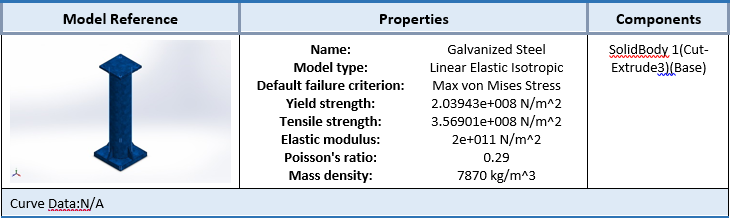
\includegraphics[scale=0.7]{material_properties}
	\caption{Solidworks definition for the material mechanical properties.}
\end{figure}



\begin{figure}[H]
	
	\centering
	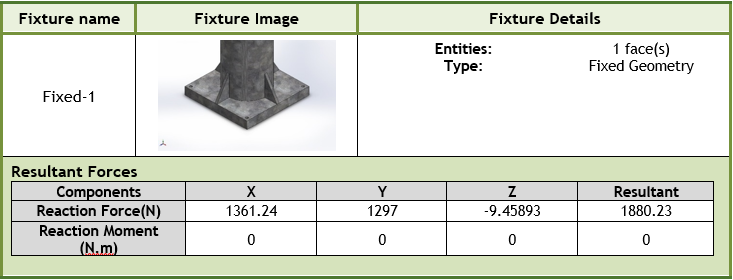
\includegraphics[scale=0.7]{load_And_fixture}
	\caption{Solidworks model reactions acting on the flange in x, y, and z.} 
\end{figure}


\begin{figure}[H]
	\centering
	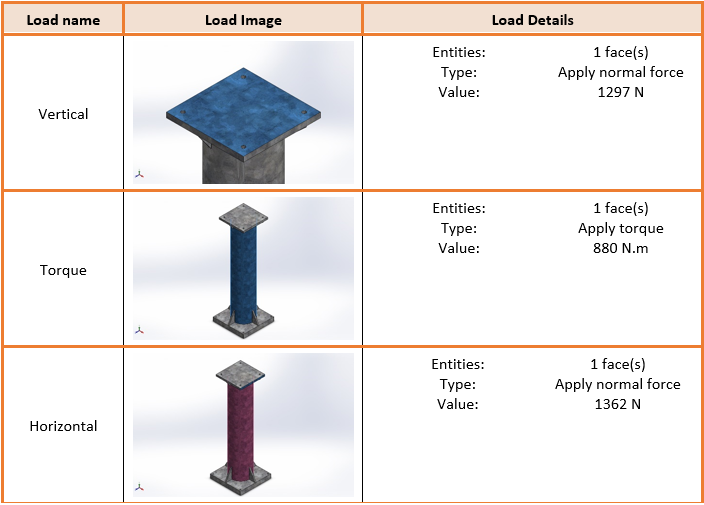
\includegraphics[scale=0.7]{load}
	\caption{Solidworks representation for different loads acting on the whole cylinder} 
\end{figure}

\begin{figure}[H]
	\centering
	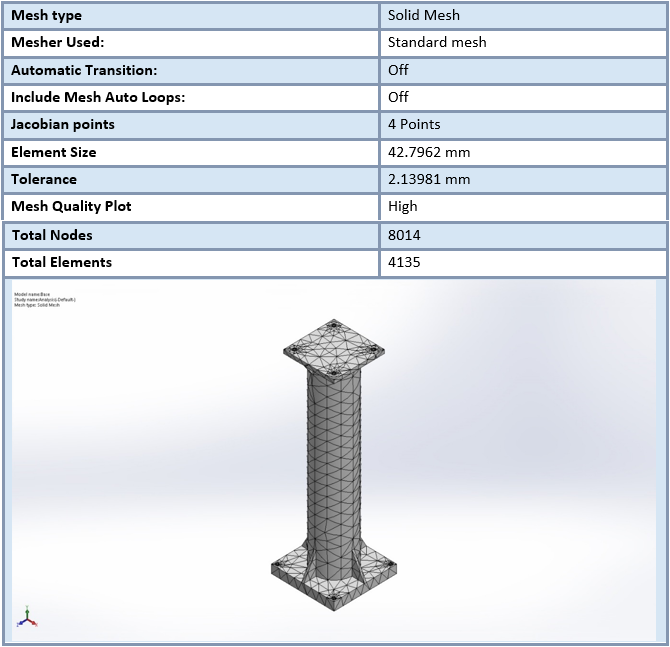
\includegraphics[scale=0.6]{mesh3}
	\caption{Mesh information obtained from Solidworks} 
\end{figure}

\begin{figure}[H]
	\centering
	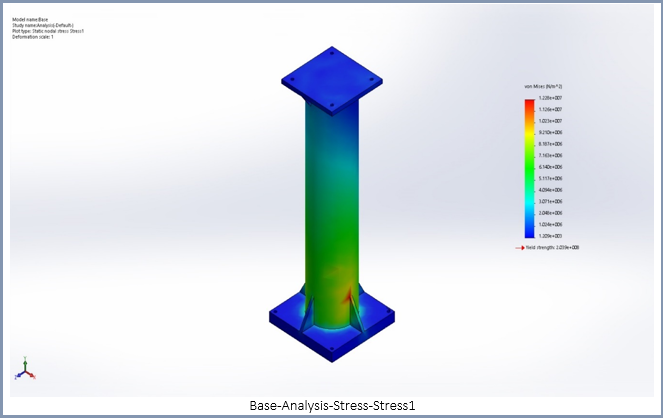
\includegraphics[scale=0.45]{zstress}
	\caption{Solidworks representation for stresses acting on the base.} 
\end{figure}
\begin{center}
	The maximum stress is 10.34 $N$/$m^{2}$ and the minimum stress is 6.8 $N$/$m^{2}$ .
\end{center}

\begin{figure}[H]
	\centering
	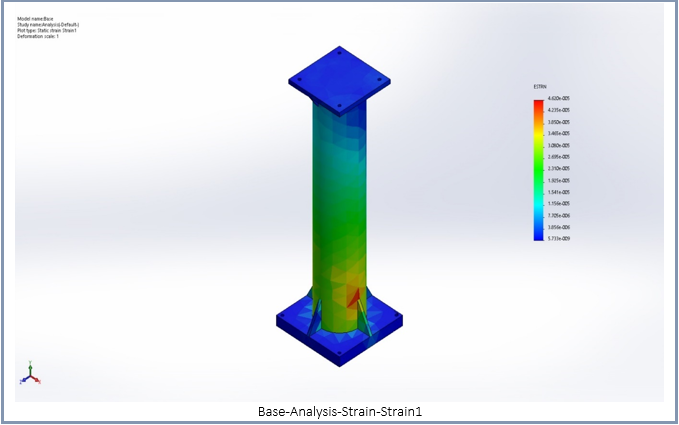
\includegraphics[scale=0.45]{zstrain}
	\caption{Solidworks representation for the base strain.} 
\end{figure}
\begin{center}
	The maximum strain is 7.56 and the minimum strain is 6.58.
\end{center}
\begin{figure}[H]
	\centering
	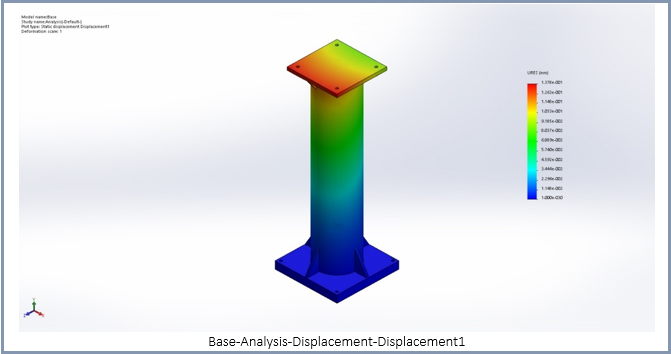
\includegraphics[scale=0.45]{zDisplacement}
	\caption{Solidworks representation for displacement at maximum loading.} 
\end{figure}
\begin{center}
	 Displacement of the base due to this forces is 2.7mm at maximum.
\end{center}


\newpage
\section{2.4 CAD Analysis Approach}

In Simulation and Analysis, you can test your designed product in real environment.In simulation process the model can be tested against parameters like static and dynamic response, fluid dynamic, heat transfer. It also supports thermal, fatigue, structural and motion analysis. 
\newline In our project, SolidWorks is used to obtain a CAD model for KR6 r900 sixx and to perform a motion analysis study on the model. In addition to designing a base to fix the robot arm, perform a stress analysis and creating an animation video of the model’s motion.

\subsection{Complete CAD Model}

\subsubsection{Searching for a suitable model}
All CAD models for KR6 r900 sixx on KUKA website or GrabCAD were step imported parts which are treated as a one body where joints can’t rotate therefore, motion study can’t be performed because it was impossible to add motors at the robot joints. The solution for this issue was obtained by converting step parts into assembly, which is done through several steps:
\begin{itemize}
	\item Open the .stp file part in SOLIDWORKS.  Select the file type to be .stp
	\item Click the OPTIONS tab, select Import multiple bodies as parts and click OK.
	\item Then click Open.
\end{itemize}
SolidWorks will create an assembly and create an individual part file for each multibody (Part1,Part2,Part3 etc.)
\begin{figure}[H]
	\centering
	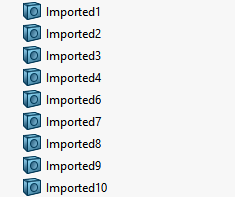
\includegraphics{Stepparts}
	\caption{Step parts}
\end{figure}

\begin{figure}[H]
	\centering
	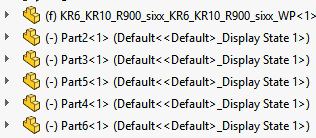
\includegraphics{assemblyparts}
	\caption{SolidWorks parts}
\end{figure}

\subsubsection{Modifications on CAD model}
\paragraph{Material and weights}
The robot material wasn’t specified and the model was a whole body, and the total mass for the robot was 33.74 Kg, which was not accurate, because the actual mass of the robot, according to the KR6 R900 sixx dimensions manual, must be approximately equal to 52Kg. This is achieved by making the model hollow, using the shell feature and adding to joins point masses similar to the real motors with mass approximate equal to motors masses. 

\begin{figure}[H]
	\centering
	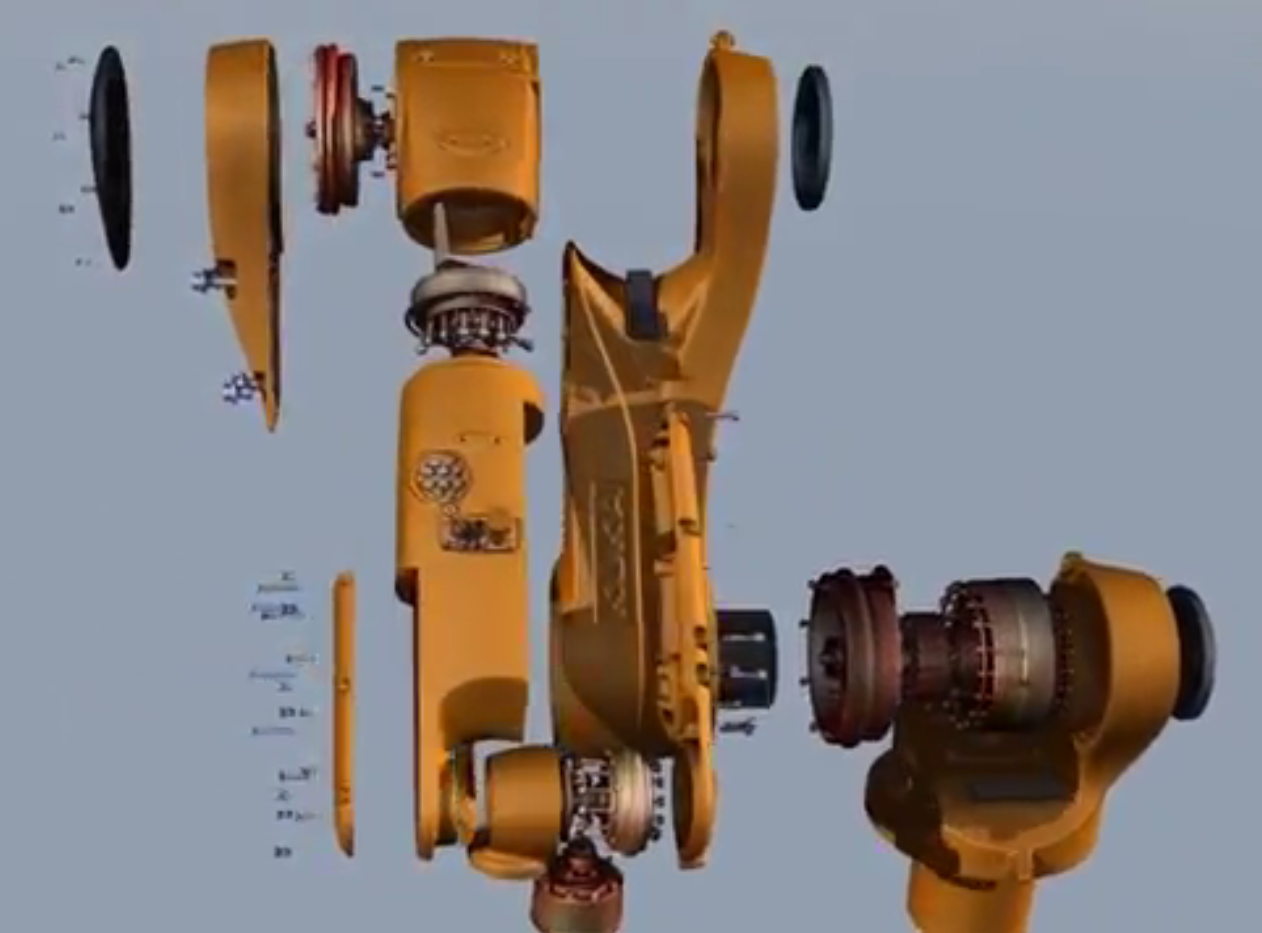
\includegraphics[scale=0.3]{KUKAmotor}
	\caption{KUKA motors}
\end{figure}

\begin{figure}[H]
		\centering
		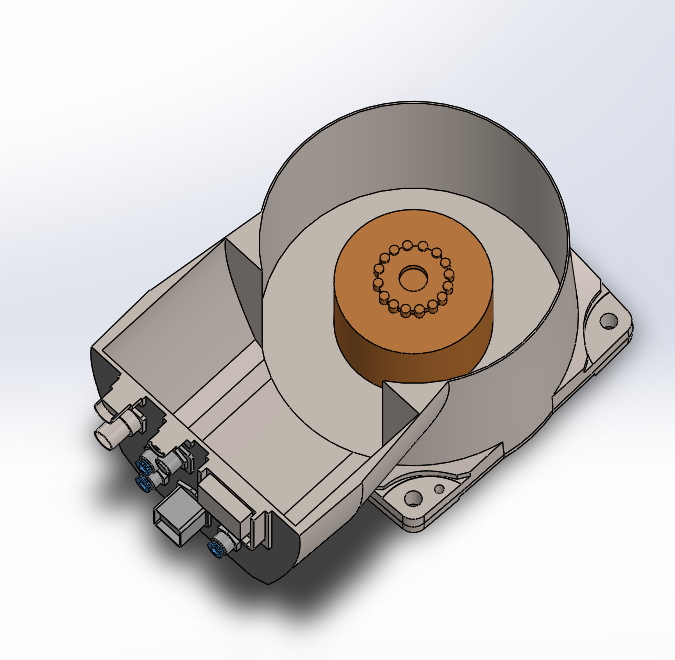
\includegraphics[width=0.6\linewidth]{Motor1}
		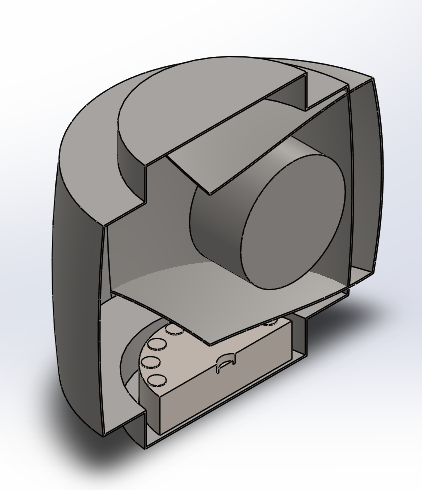
\includegraphics[width=0.4\linewidth]{Motor3}
	\caption{Motors model: Motors 1,2 and 3 model and Motors 4,5 and 6 model}
	\label{fig:fig}
\end{figure}

\begin{figure}[H]
		\centering
		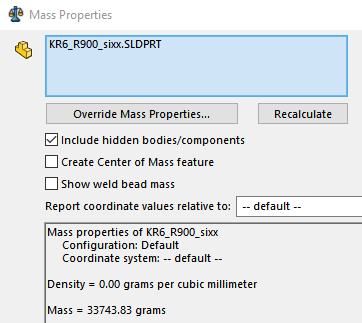
\includegraphics[width=0.6\linewidth]{Massbeforeadjust}
		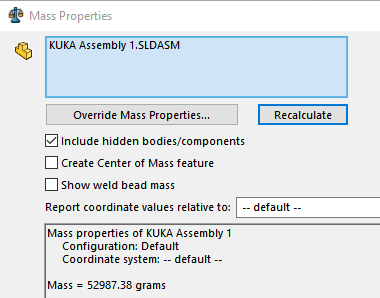
\includegraphics[width=0.45\linewidth]{Finalmass}
	\caption{The model mass: Old mass and final mass}
	\label{fig:fig22}
\end{figure}

\paragraph{Spindle}
In order to have a complete model for our graduation project, a router spindle and its holder were sketched to complete the existing KUKA model.

\begin{figure}[H]
	\centering
	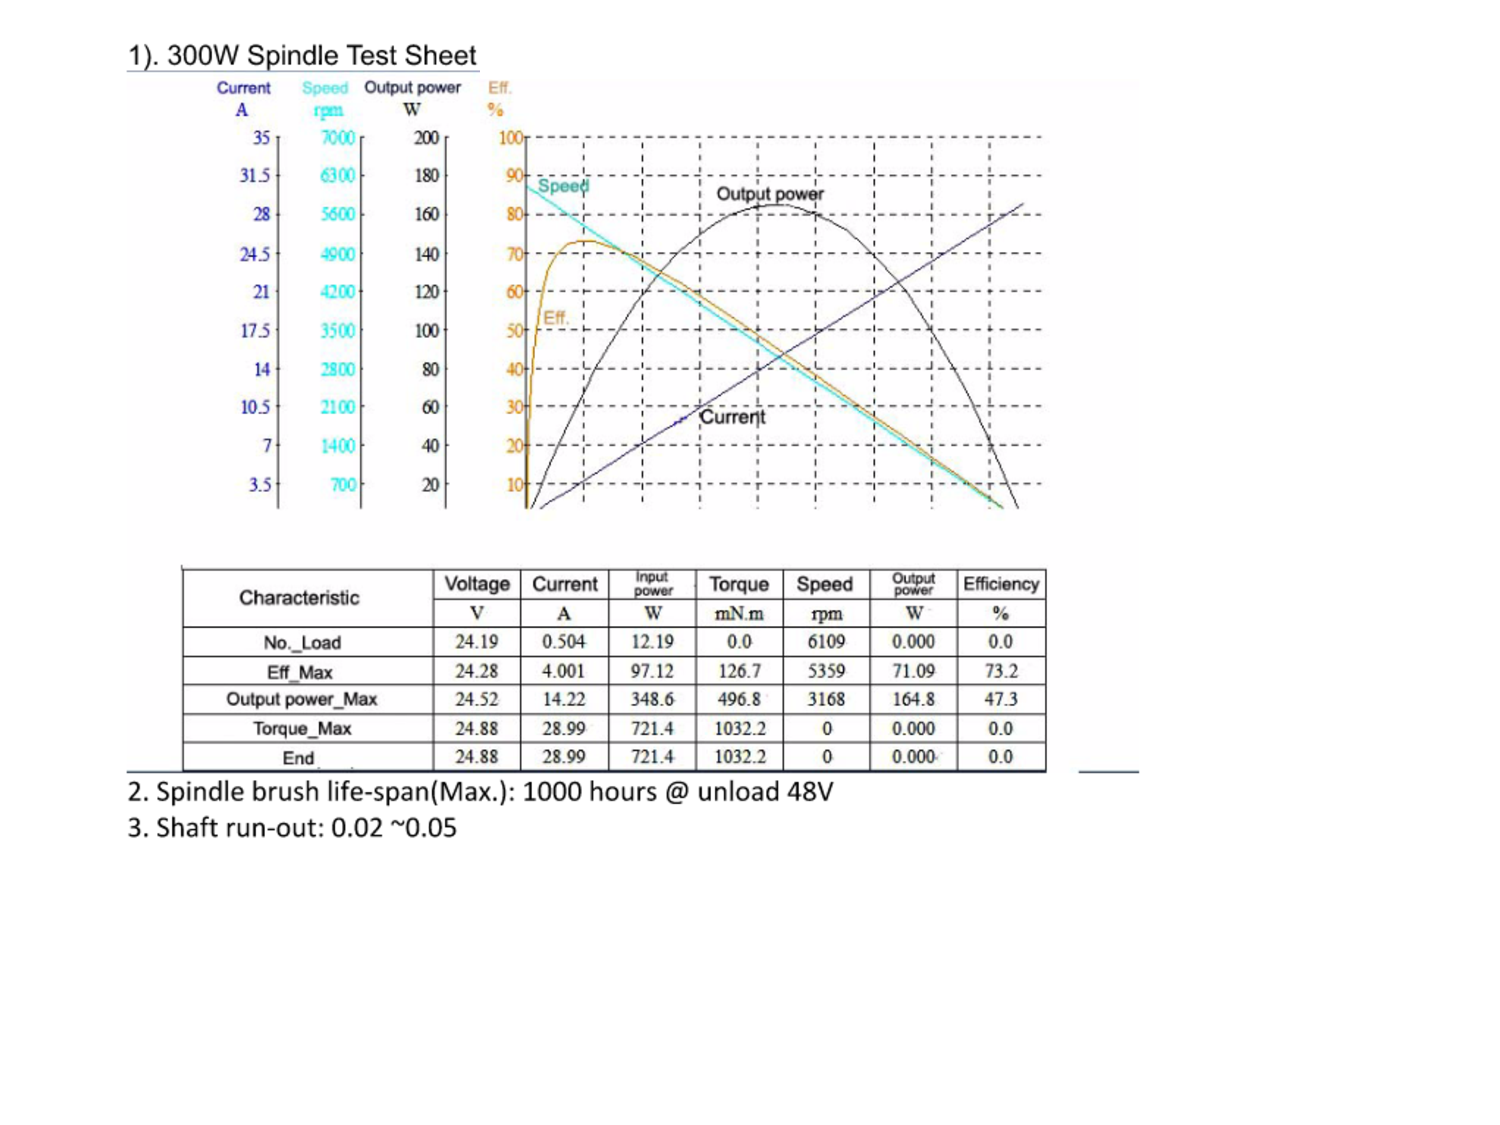
\includegraphics[scale=0.2]{spindle}
	\caption{Spindle model}
\end{figure}

\begin{figure}[H]
	\centering
	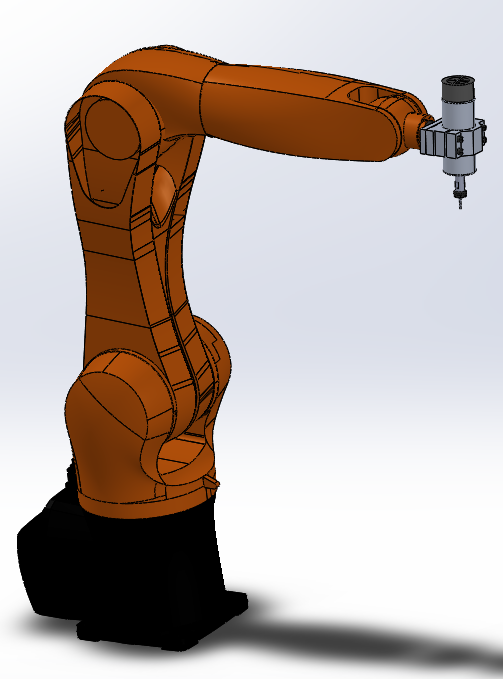
\includegraphics[scale=0.45]{FinalCADmodel}
	\caption{Final CAD model}
\end{figure}

\subsection{Motion studies}
Motion studies are graphical simulations of motion for assembly models. They simulate and animate the prescribed motion for a model. SolidWorks offer three different types of motion study, Animation, Basic Motion and Motion Analysis. They also offer mate controller that show, save the positions of assembly components at various mate values and degrees of freedom and create simple animations between those positions.
\smallskip
\newline Animation can be used to animate the motion of assembly. If you simply wish to create some nice visuals for presentation or marketing without consideration of mass and gravity effects, then animation is for you. 
\newline Basic Motion is an extra layer of complexity that takes into consideration the effects of mass, motors, springs, contact, and gravity on assemblies. 
\smallskip
\newline Motion Analysis is the top tier of motion study provides accurately simulation and analyze the motion of an assembly while incorporating the effects of Motion Study elements (including forces, springs, dampers, and friction). Motion Analysis can also be used to plot simulation results for further analysis.
\smallskip
\newline Therefore, Motion Analysis is used to simulate the model, generating results and plots of the simulation and Animation is used to make a video for motion.

\bigskip
\subsubsection{Animation study} 
Animation study is done to make an animation video of the moving parts with the use of limit mates. Limit angle mate is an advanced mate type that is performed by selecting two planes which rotate with respect to each other giving the desired range to mate and input a maximum and minimum value for the angle to specify the desired range of motion. Another advantage of limit angle is that it prevent collision between the moving parts.

\begin{figure}[H]
	\centering
	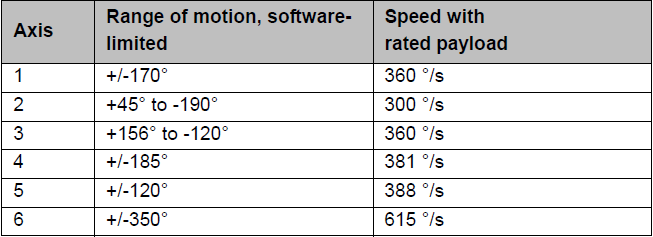
\includegraphics[scale=0.7]{Axesrangeofmotion}
	\caption{Axes range of motion}
\end{figure}

\bigskip
\subsubsection{Motion analysis}
On implementing motion analysis by adding a motor at the required location to start simulating the robot, a problem arose; the model exploded on running the simulation where some of the parts were separated from each other. This happened because of redundancy constrains. For Motion Analysis studies, having redundant mates is the equivalent of over-defining the model.  

\begin{figure}[H]
	\centering
	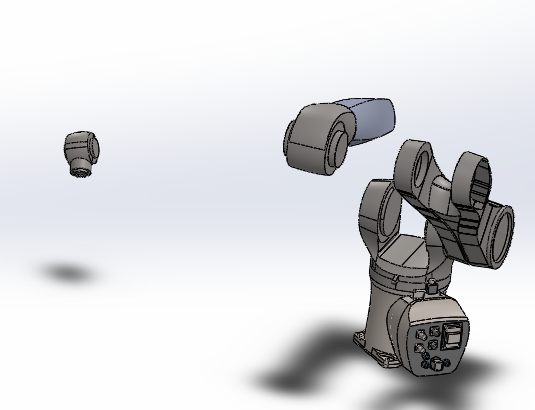
\includegraphics[scale=0.45]{Redundancyproblem}
	\caption{Redundancy constraint problem}
\end{figure}

This issue was solved by using mechanical mates of hinge type instead of standard mates. Hinge mate limits the movement between two components to one rotational degree of freedom. It has the same effect as adding a concentric mate plus a coincident mate and also limit the angular movement between the two components by adding limit angles. Reducing the negative effect of redundant mates on analysis.

\begin{figure}[H]
	\centering
	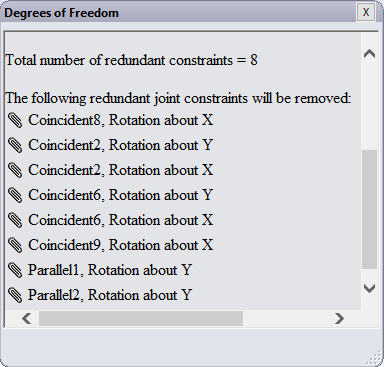
\includegraphics[scale=0.6]{redundancyconstrains}
	\caption{Presence of redundancy constrains}
\end{figure}

\begin{figure}[H]
	\centering
	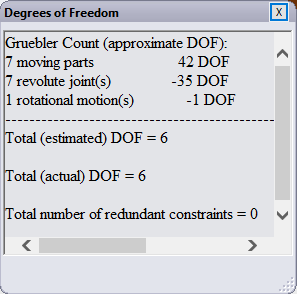
\includegraphics[scale=0.9]{zeroredandantcontraints}
	\caption{Zero redundant constraints}
\end{figure}
\smallskip
Now motors can be added to the model to perform any motion and results as motor torque, velocity, acceleration and force are generated.

\bigskip
\paragraph{Results of motion analysis study}] 
By assigning a motor to simulate the motion of axis and plotting the results to achieve this motion we found:
\begin{enumerate}
	\item Results of motor torque for axis 1 to move 100 degrees in 4 seconds:

	\begin{figure}[H]
		\centering
		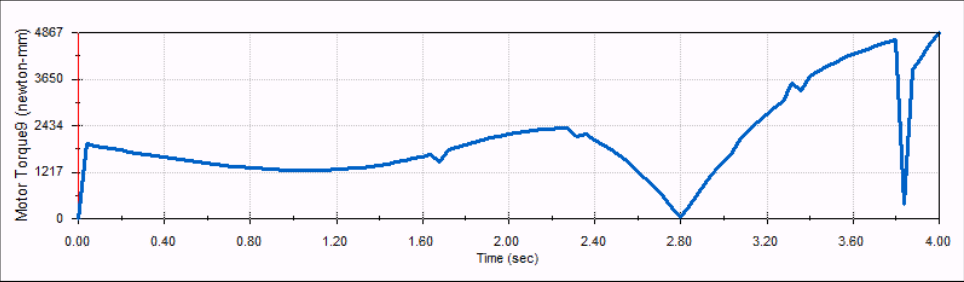
\includegraphics[scale=0.5]{Motor1torque}
		\caption{Motor 1 torque}
	\end{figure}
	
	\smallskip
Knowing that the actual motor torque for axis 1 is 4.5 N.m so the motion analysis result is approximate to actual torque. 
\newline Motor torque vary with time because of the motion of the links beyond the motor which has an effect on the torque by changing the loads carried by the motor.
\smallskip
	\item Motor 2 torque to move 60 degrees in 2 seconds:
	\begin{figure}[H]
		\centering
		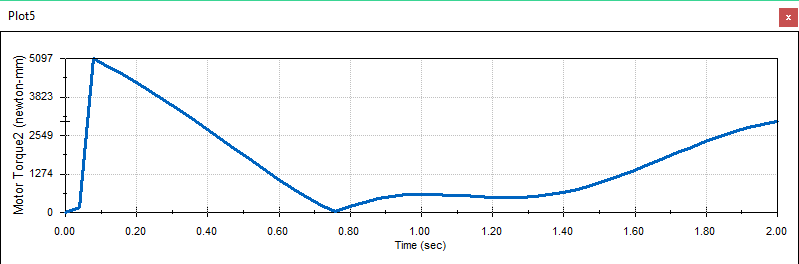
\includegraphics[scale=0.6]{Motor2torque}
		\caption{Motor 2 torque}
	\end{figure}
	
	Where the actual motor torque is 4 N.m

\smallskip
	\item Motor torque for axis 3 to move 75 degrees in 1.8 seconds:
	\begin{figure}[H]
		\centering
		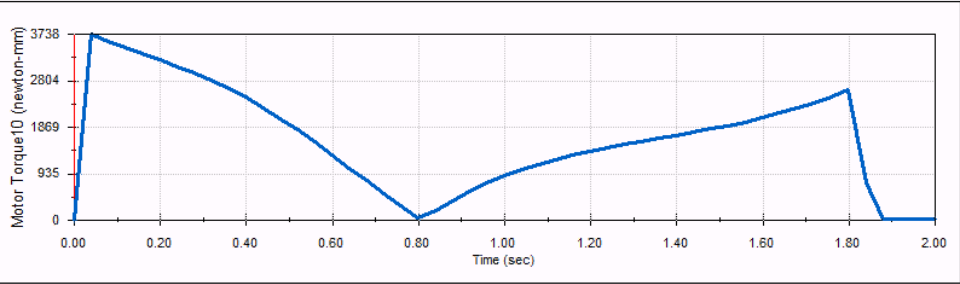
\includegraphics[scale=0.45]{Motor3torque}
		\caption{Motor 3 torque}
	\end{figure}
	
	Knowing that the actual motor torque for axis 3 is 3.5 N.m so the motion analysis result is approximate to actual torque.
\end{enumerate}

\bigskip
\paragraph{Trace path}
Motion analysis results and plots have a trace path option that can trace the path of a point in the assembly. The selected point is end mill vertex to create the curve feature that represent the motion of the links.  By assigning a data point motors to the joints whose data is imported from excel spreadsheet of file type .csv containing two columns, first represent time in seconds while other is degrees of rotation. The generated curve of adding this data to joints 1-5 is an arc shape.

\begin{figure}[H]
	\centering
	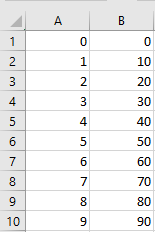
\includegraphics[scale=0.6]{datapoint}
	\caption{Used data point}
\end{figure}

\begin{figure}[H]
	\centering
	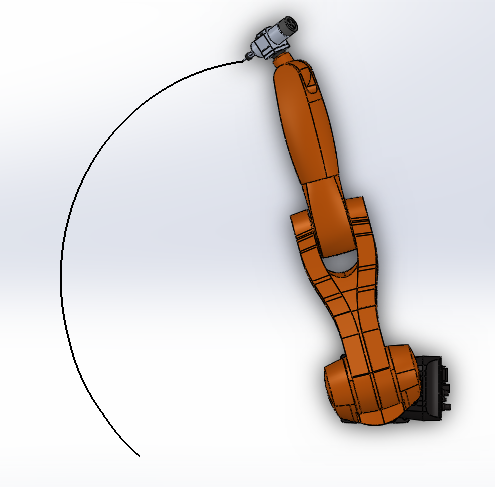
\includegraphics[scale=0.6]{Tracepathcurve}
	\caption{Created curve}
\end{figure}

%
%\end{chapter}
%    \end{document}